% Emacs, this is -*- latex -*-!
% Ensure that arXiv processes this as PDF.
\pdfoutput=1

\documentclass{sigplanconf}

% Emacs, this is -*- latex -*-!
\usepackage{natbib}
\usepackage{rotating}
\usepackage{amsmath}
\usepackage{comment}
\usepackage[shortlabels]{enumitem}
\usepackage[T1]{fontenc}
\usepackage[utf8]{inputenc}
\usepackage{xparse}
\usepackage{microtype}

\usepackage{subcaption}

% This package allows hyphenation of compound words. Use \-/
% instead of - as hyphen to allow hyphenation elsewhere. Use \=/
% to additionally specify that hyphenation right after the dash
% is forbidden. However, this package with this setting redefines
% \- and \=!

%\usepackage[shortcuts]{extdash}

\usepackage{etoolbox} %For newtoggle
\newtoggle{todos}

% Show empty space at page ends, to ease squeezing space.
% Should remove before submission.
%\raggedbottom

% For submission. These settings shouldn't be altered.
\togglefalse{todos}
% \toggletrue{todos}
\allowdisplaybreaks[1]
% For development, feel free to tune if needed.
% Allow reasonable looks without huge cost, during development.
%   \allowdisplaybreaks[1]
%   %\sloppy

% Introduce environment oldSec for material which we commented out but might
% still have bits to save:
\excludecomment{oldSec}
% Replace the above line with:
%\includecomment{oldSec}
% to comment those sections back in.
\newenvironment{optionalproof}{\begin{proof}}{\end{proof}}
\newenvironment{optionallemma}{\begin{lemma}}{\end{lemma}}


%%%%%%%%%%%%%%%%%%%%%%%%%%%%%%%%%%%%%%%%%%%%
% SIGPLANconf-specific setup
%
% amsthm conflicts with LLNCS.
%%%%%%%%%%%%%%%%%%%%%%%%%%%%%%%%%%%%%%%%%%%%
\usepackage{amsthm,listings,fixfoot}
% Hey Emacs this is -*- latex -*-
% From http://tihlde.org/~eivindw/latex-listings-for-scala/
% "define" Scala
%Keyword list taken from the scaladoc definition.
\lstdefinelanguage{scala}{
  morekeywords={%
	  abstract,case,catch,class,def,do,else,extends,%
	  false,final,finally,for,forSome,if,implicit,import,lazy,%
	  match,new,null,object,override,package,private,protected,%
	  return,sealed,super,this,throw,trait,true,try,type,%
	  val,var,while,with,yield},
  otherkeywords={=>,<-,<\%,<:,>:,\#,@,scala>},
  sensitive=true,
  morecomment=[l]{//},
  morecomment=[n]{/*}{*/},
  morestring=[b]",
  morestring=[b]',
  morestring=[b]"""
}[keywords,comments,strings]

% activate the language and predefine settings
\lstset{%
    language=Scala,%
    tabsize=2,%
    basicstyle=\ttfamily,%
    commentstyle=\itshape,%
    keywordstyle=\bfseries,%
    identifierstyle=,% nothing
    stringstyle=\ttfamily, % typewriter type for strings
    mathescape=true,%
    escapechar=£,%
    numberstyle=\tiny,%
}

%Setup whitespace in listings
\lstset{%
%columns=fullflexible,		% enable kerning, lose column alignment.
showstringspaces=false, %
breaklines=false,
breakatwhitespace=false,
breakautoindent=false,
keepspaces
%keepspaces was described at: http://tex.stackexchange.com/questions/41954/listings-bug-space-after-literate-replacement-lost-with-spaceflexible-fullflexi
}

\newcommand{\codesize}{}

% Command for in-text code snippets, if needed.
\newcommand{\code}{%
    \lstinline[basicstyle=\codesize\ttfamily]}

% I use ^ as the only decent alternative - not-ASCII characters don't work in this setup (probably because of UTF-8).}
% literate programming: replace some operators by nicer equivalents.
%{==}{{$\equiv$}}1 {!=}{{$\neq$}}1
\lstset{literate={{<-}{{$\gets$}}1 {<=}{{$\leq$}}1 {>=}{{$\geq$}}1 { => }{{$\Rightarrow$}}1 { -> }{{$\rightarrow$}}1 {...}{{\ldots} }2}}



% The next package must be loaded last.
% It adds the \cref{label} command, producing Eq./Sec./whatever followed by the reference.
\usepackage[capitalise]{cleveref}

\crefname{section}{Sec.}{Sec.}
\crefname{subsection}{Sec.}{Sec.}
\crefname{subsubsection}{Sec.}{Sec.}


% Theorems, lemmas, corollaries
% Typeset in roman to avoid known TeX feature
% (bad spacing between italic text and math formulas)
%
% Numbering:
% Theorem 3.1. It always rains.
% Lemma 3.2. If it rains, then the weather is bad.
% Corollary 3.3. The weather is always bad.
%
% http://tex.stackexchange.com/a/67251
\theoremstyle{definition}
\input QED
\newtheorem{theorem}{Theorem}[section]
\newtheorem{lemma}[theorem]{Lemma}
\newtheorem{corollary}[theorem]{Corollary}
\newtheorem{definition}[theorem]{Definition}

\begin{oldSec}
\newtheorem{parameter}[theorem]{Plugin Requirement}
\end{oldSec}

%%%%%%%%%%%%%%%%%%%%%%%%%%%%%%%%%%%%%%%%%%%%
% Enumerations inside theorem environments
%
% (cannot be in macros.tex because of \crefname)
%%%%%%%%%%%%%%%%%%%%%%%%%%%%%%%%%%%%%%%%%%%%

\newlist{subdefinition}{enumerate}{1}
\setlist*[subdefinition]{label=(\alph*), ref=\arabic{section}.\arabic{theorem}\alph*}
\crefname{subdefinitioni}{Property}{Properties}
\Crefname{subdefinitioni}{Property}{Properties}

\newlist{subparameter}{enumerate}{1}
\setlist*[subparameter]{label=(\alph*), ref=\arabic{section}.\arabic{theorem}\alph*}
\crefname{subparameteri}{Plugin Requirement}{Plugin Requirements}
\Crefname{subparameteri}{Plugin Requirement}{Plugin Requirements}

\newlist{subtheorem}{enumerate}{1}
\setlist*[subtheorem]{label=(\alph*), ref=\arabic{section}.\arabic{theorem}\alph*}
\crefname{subtheoremi}{Theorem}{Theorems}
\Crefname{subtheoremi}{Theorem}{Theorems}

% Our project
\newcommand{\ILC}{I{\TitleLambda}C}

\begin{document}


%%%%%%%%%%%%%%%%%%%%%%%%%%%%%%%%%%%%%%%%%%%%
% Paper information in SIGPLANconf-style
%%%%%%%%%%%%%%%%%%%%%%%%%%%%%%%%%%%%%%%%%%%%

\conferenceinfo{PLDI '14}{June 9--11, 2014, Edinburgh, UK}
\copyrightyear{2014}
\copyrightdata{[to be supplied]}

\title{A Theory of Changes for Higher-Order Languages}
\subtitle{Incrementalizing {\TitleLambda}-Calculi by Static Differentiation}

% Alternatives:
%
% (Incremental Computation for | Incrementalizing) (the Lambda
% Calculus | (Higher-Order | First-Class) Functions)

\iftoggle{names}{%
\newcommand{\unimarburg}{Philipps-Universität Marburg}
\authorinfo{Yufei Cai}
           {\unimarburg}{}
\authorinfo{Paolo G. Giarrusso}
           {\unimarburg}{}
\authorinfo{Tillmann Rendel}
           {\unimarburg}{}
\authorinfo{Klaus Ostermann}
           {\unimarburg}{}
}{%
\authorinfo{}
           {}{}
}

\maketitle

\begin{abstract}
% Emacs, this is -*- latex -*-!
If the result of an expensive computation is invalidated by a small
change to the input, the old result
should be updated incrementally instead of reexecuting the whole computation.
We incrementalize programs through
their \emph{derivative}. A derivative maps
changes in the program's input directly to changes in the program's
output, without reexecuting the original program. We present a
program transformation taking programs to their
derivatives, which is fully static and automatic, supports first-class
functions, and produces derivatives amenable to standard
optimization.

We prove the program transformation correct in Agda for a
family of simply-typed $\lambda$-calculi, parameterized by base
types and primitives. A precise interface specifies what is
required to incrementalize the chosen primitives.

We investigate performance by a case study: We implement in Scala the
program transformation, a plugin and improve performance of a nontrivial program by
orders of magnitude.

% \pg{Failed attempt at four-sentence abstract. Our paper isn't that cool yet. Hmpf!}
% \pg{I submitted what's above for now. But maybe we should still try to have
% something like this?}
% Results of expensive computations are often recomputed from scratch when
% the input changes. Often, this wastes time because changes are
% small and the output could be updated much faster; writing
% code performing efficient updates by hand is error-prone. We propose
% a program transformation taking a program to its
% \emph{derivative}, mapping changes to inputs to changes to
% outputs, often more efficiently, and we perform case studies
% showing significant performance improvements.

\keywords
Incremental computation, first-class functions, performance, Agda, formalization
\end{abstract}

% TODO: Readd in camera-ready version, usually not needed before.
%\category{CR-number}{subcategory}{third-level}
%
%\terms
%term1, term2
%
%\keywords
% Keywords.

%%%%%%%%%%%%%%%%%%%%%%%%%%%%%%%%%%%%%%%%%%%%
% Paper body
%%%%%%%%%%%%%%%%%%%%%%%%%%%%%%%%%%%%%%%%%%%%

% Invariant: Each inclusion corresponds to a top-level section.
% Emacs, this is -*- latex -*-!

\section{Introduction}
\label{sec:intro}

Incremental computation has a long-standing history in computer
science~\citep{Ramalingam93}. Often, a program needs to update its
output efficiently to reflect input
changes~\citep{Salvaneschi13reactive}. Instead of rerunning such a
program from scratch on its updated input, incremental
computation research looks for alternatives that are cheaper in a common scenario:
namely, when the input change is much smaller than the input itself.

For instance, consider the $\Program$ program, which calculates
the sum of all numbers in collections $\Xs$, $\Ys$.
\begin{align*}
\Program & = \ProgramBody\\
\Output & = \Program~\Set{1,1}~\Set{2,3,4}=11
\end{align*}
With $\Set{\ldots}$ we represent a multiset or \emph{bag}, that is an unordered collection (like a set)
where elements are allowed to appear more than once (unlike a set).
Now assume that the input $\Xs$ changes from $\Set{1,1}$ to
$\Set{1}$, and $\Ys$ changes from $\Set{2,3,4}$ to $\Set{2,3,4,5}$.
Instead of recomputing $\Output$ from scratch, we could also compute it incrementally. If we have a
representation for the changes to the inputs (say,
$\DXs = \Set{\Keyword{remove} \; 1}$,
$\DYs = \Set{\Keyword{add} \; 5}$), we can compute the new
result through a function $\Derivative$ that takes the old inputs
$\Xs = \Set{1,1}$, $\Ys=\Set{2,3,4}$ and the changes $\DXs$,
$\DYs$ to produce the output change.
In this case, it would compute the change
$\Derivative~\Xs~\DXs~\Ys~\DYs = \Keyword{plus} \; 4$,
which can then be used to update the original output $11$
%
to yield the updated result $15$. We call $\Derivative$ the \emph{derivative} of $\Program$.
It is a function in the
same language as $\Program$, accepting and producing changes, which
are simple first-class values of this language.
%
If we increase the size of the original inputs $\Xs$ and $\Ys$, the time
complexity of $\Program~\Xs~\Ys$ increases linearly, while the time complexity
of $\Derivative~\Xs~\DXs~\Ys~\DYs$ only depends on the size of $\DXs$ and $\DYs$,
which is smaller both in our example and in general.

To support automatic incrementalization, in this chapter we introduce the \ILC\
(incrementalizing $\Gl$-calculi) framework. We define
an automatic program transformation $\DERIVE$
that \emph{differentiates} programs, that is, computes their
derivatives; $\DERIVE$ guarantees that
\begin{equation}
  \label{eq:correctness}
\App{f}{\Apply*{\D a}{a}}
\cong
\Apply{\App*{\App{\Derive{f}}{a}}{\D a}}{\App*{f}{a}}.
\end{equation}
where
$\cong$ is denotational equality,
$\D a$ is a change on $a$ and $\Apply{\D a}{a}$ denotes $a$
updated with change $\D a$, that is, the updated input of $f$.
Hence, we can optimize programs by replacing the left-hand side,
which recomputes the output from scratch, with the right-hand
side, which computes the output incrementally using derivatives.
% KO: I think this forward references confuses more than it helps.
%Our approach relates to \emph{finite differencing} but has a more
%general theory and support for first-class functions (see
%\cref{sec:finite-diff}).

\ILC\ is based on a simply-typed $\Gl$-calculus
parameterized by \emph{plugins}. A plugin
defines
%
(a) base types and primitive operations, and
%
(b) a change representation for each base type, and an
incremental version for each primitive. In other words, the plugin
specifies the primitives and their respective derivatives, and
\ILC\ can glue together these simple derivatives in such a way
that derivatives for arbitrary simply-typed $\Gl$-calculus expressions
using these primitives can be computed. Both our implementation and our correctness proof 
is parametric in the plugins, hence it is easy to support (and prove correct)
new plugins.

This chapter makes the following contributions:
\begin{itemize}
\item We present a novel mathematical theory of changes and derivatives, which is more
  general than other work in the field because changes are
  first-class entities, they are distinct from base values and
  they are defined also for functions (\cref{sec:1st-order-changes}).
  %KO: I think the next sentence cannot be understood at this point.
  %We introduce changes for complex types, defined compositionally.
%
\item We present the first approach to incremental computation for
pure $\lambda$-calculi by a source-to-source transformation, $\DERIVE$, that requires no run-time
support. The transformation produces an incremental program in the same language;
all optimization techniques for the original program are
applicable to the incremental program as well.
%KO: commented this out. I think the purity is not important enough
%to deserve another sentence here, since we only vaguely hint
%at "further research".
%Since our incremental programs use no impure features, they are
%especially amenable to further optimizations, making this approach
%very suitable for further research.
%
% KO: Let's have one bullet point per section. Also, a conjecture
% sounds like a rather weak contribution
%\item We argue that incrementalization is efficient on
%  \emph{self-maintainable programs}, and discuss how further research on
%  static or dynamic memoization can speed up a larger class of programs (\cref{sec:performance-cons}).
%  \pg{This contribution references text which is now commented
%    out. I believe the text should be brought back in.}
%
We prove that our incrementalizing transformation $\DERIVE$
is correct~(\cref{eq:correctness})
by a machine-checked formalization in Agda~\citep{agda-head}.
The proof gives insight into the definition of $\DERIVE$: we
first construct the derivative $\EvalInc{-}$ of the denotational
semantics of a simply-typed $\lambda$-calculus term, that is, its
\emph{change semantics}.
%
Then, we show that $\DERIVE$ is produced by erasing
$\EvalInc{-}$ to a simply-typed program (\cref{sec:correctness}).

\item While we focus mainly on the theory of changes
and derivatives, we also perform a performance case study.
We implement the derivation transformation in Scala,
with a plug-in architecture that can be extended with new base
types and primitives. We define a plugin with support for
different collection types and use the plugin to 
incrementalize a variant of the MapReduce programming model~\citep{Lammel07}.
  Benchmarks show that on this program,
  incrementalization can reduce asymptotic complexity and can turn $O(n)$
  performance into $O(1)$, improving running time by over 4
  orders of magnitude on realistic inputs (\cref{sec:applying}).

\end{itemize}

% KO: We said all that is in this paragraph before.
% Our formalization is generic in the set of base types and the set
% of primitives that operate on these base types. That is, we
% present only the core of the formalization that deals with
% function types, lambda abstraction, application and variable
% references. Base types and primitives on base types have to be
% added as plugins. The interface between the core formalization
% and the plugins is formalized as well. It consists of the sets,
% operations, and lemmas that a plugin has to provide in order to
% fit into the core formalization. We hope that the generic
% formalization allows us and other researchers to experiment with
% different choices of base types, and different incrementalization
% strategies for these base types.

%We mechanized the formalization, including the separation between
%core and plugins, in the dependently typed programming language
%Agda~\cite{agda-head}.
Our Agda formalization, Scala implementation and benchmark
results are available at the URL
\url{http://inc-lc.github.io/}.
All lemmas and theorems presented
in this chapter have been proven in Agda.
In the chapter, we present an overview of
the formalization in more human-readable form, glossing over some
technical details.

% KO: Old stuff which contains snippets to be integrated in other sections, in 
% particular Related Work.


% Emacs, this is -*- latex -*-!
%\section{Changes as First-Class Values}
\section{A theory of changes}
\label{sec:1st-order-changes}

This section introduces a formal concept of changes; this
concept was already used informally in \cref{eq:correctness} and is central
to our approach. We first define change structures formally, then construct 
change structures for functions between change structures,
and conclude with a theorem that relates function changes to derivatives. 

\subsection{Change structures}\label{ssec:change-structures}
Consider a set of values, for instance the set of natural numbers
$\mathbb{N}$. A change $\D v$ for $v \in \mathbb{N}$ should
describe the difference between $v$ and another natural $\New{v}
\in \mathbb{N}$. We do not define changes directly, but we
specify operations which must be defined on them. They are:
\begin{itemize}
\item We can \emph{update} a base value $v$ with a
  change $\D v$ to obtain an updated or \emph{new} value
  $\New{v}$. We write $\New{v} = \Apply{\D v}{v}$.
\item We can compute a change between two arbitrary
  values $\Old{v}$ and $\New{v}$ of the set we are considering.
  We write $\D v = \Diff{\New{v}}{\Old{v}}$.
\end{itemize}

For naturals, it is usual to describe changes using standard
subtraction and addition. That is, for naturals we can define
$\Apply{\D v}{v} = v + \D v$ and $\Diff{\New{v}}{\Old{v}} =
\New{v} - \Old{v}$. To ensure that $\APPLY$ and $\DIFF$ are
always defined, we need to define the set of changes carefully.
$\mathbb{N}$ is too small, because subtraction does not always
produce a natural; the set of integers $\mathbb{Z}$ is instead
too big, since adding a natural and an integer does not always
produce a natural. In fact, we cannot use the same set of all
changes for all naturals. Hence we must adjust the requirements:
for each base value $v$ we introduce a set $\Change{v}$ of
changes for $v$, and require $\Diff{\New{v}}{\Old{v}}$ to produce
values in $\Change{\Old{v}}$, and $\Apply{\D v}{v}$ to be defined
for $\D v$ in $\Change{v}$. For natural $v$, we set $\Change{v} =
\left\{\D v \mid v + \D v \geq 0 \right\}$; $\DIFF$ and $\APPLY$ are
then always defined.

\begin{oldSec}

\ldots, we could use \emph{functional
changes}, that is by defining changes to be functions from the
old value to the new value:
\begin{align*}
\Change{\Gt} & = \Gt \r \Gt, \\
\Apply{\D v}{\Old{v}} & = \App{\D v}{\Old{v}},\\
\Diff{\New{v}}{\Old{v}} & = \Lam{x}{\New{v}}.
\end{align*}
However,
this definition does not allow derivatives to analyze changes to
be more efficient than recomputation. To understand why, let us
consider the following example.

Let $\Old{v} = \{1, 2, \ldots, n\}$ be a bag (or multiset) of
integers, let $f$ be a function from bags to integers summing the
elements of its argument, and let $\Old{s} = \App{f}{\Old{v}}$.

Later during program execution, assume we add $n + 1$ to
$\Old{v}$ and need to update $\Old{s}$. Hence,
 $\New{v} = \{1, 2, \ldots, n, n + 1\}$, $\D v$ represent the change of $v$,
and we need to compute the result of $\New{s} = \App{f}{\New{v}}$.
%
Thanks to \cref{eq:correctness}, we can guarantee that
$\New{s} = \Apply{\App{\App{\Derive{f}}{\Old{v}}}{\D
    v}}{\Old{v}}$.

Now, if $\Derive{f}$ would know that $\D v$ only added $n + 1$ to
the bag, it could produce in $O(1)$ a change $\D s$ such that
$\Apply{\D s}{s} = n + 1 + s$. But if $\D v$ is simply a function
such that $\App{\D v}{\Old{v}} = \New{v}$, we have no way of
inspecting its intension, since in $\lambda$-calculus functions
are opaque. Instead, the difference between two bags can be
described as another bag, and $\APPLY$ for bags can be defined as
bag merge.%
\footnote{Negative multiplicities are required to represent
  removals, as we discuss in Sec.~\ref{sec:plugins}.} Similarly,
we can describe the difference between two numbers $x$ and $y$ as
their arithmetical difference $x-y$. In this case, the change
application operator $\APPLY$ would be the normal addition
operator $+$. With these definitions, thanks to the structure of
$+$, $\App{\App{\Derive{f}}{\Old{v}}}{\D v}$ can produce its
result without even using $\Old{v}$, in time $O(|\D v|)$ (we
explain later how to compute $\Derive{f}$ automatically).

For now, we simply note that we cannot fix $\Change{\Gt} = \Gt \r
\Gt$. We need a more flexible encoding of changes, which allows
inspecting their structure; moreover, this structure needs to
allow writing efficient derivatives, in particular efficient
derivatives for the primitives acting on $\Gt$.

Hence, to make our general framework
independent of such domain- and application-specific
considerations, we simply require language plugins to define not
only base types and primitives for them, but also $\Change{\tau}$
whenever $\tau$ is a base type, and operators $\APPLY_\tau$ and
$\DIFF_\tau$.
Using $\APPLY$, we can recover a function $\Gt\r\Gt$
from any $\D x$ of type $\Change{\Gt}$; it is $\Lam*x{\Apply{\D
x}{x}}$.
\end{oldSec}

\pg{We never say why we use ``structure''. On second thought,
  this might be OK since we have little space.}
The following definition sums up the discussion so far:

\pg{Consider less heavyweight phrasing, such as: ``To each $v \in V$
  we associate a set of changes $\Change{v}$. But do this consistently.}
\begin{definition}[Change structures]
  \label{def:change-struct}
  A tuple $\ChangeStruct{V} = (V, \CHANGE,
  \UPDATE,
  \DIFF)$ is a \emph{change structure} (for $V$) if:

  \begin{subdefinition}
  \item $V$ is a set, called the \emph{base set}.
  \item Given $v \in V$, $\Change{v}$ is a set, called the \emph{change set}.
  \item Given $v \in V$ and $\D v \in \Change{v}$, $\Apply{\D v}{v} \in V$.
    \label{def:update}
  \item Given $u, v \in V$, $\Diff{u}{v} \in \Change{v}$.
    \label{def:diff}
  \item Given $u, v \in V$, $\Apply{\Diff*{u}{v}}{v}$ equals $u$.
    \qed
    \label{def:update-diff}
  \end{subdefinition}
\end{definition}

One might expect a further assumption that
$\Diff{\Apply*{\D v}{v}}{v} = \D v$. While it does hold
for the change structure of $\mathbb{N}$, it is not needed in general.
This means that multiple changes can represent the difference between
the same two base values. Throughout our theory, we only discuss equality of
base values, not of changes.

\paragraph{Notation}
We overload operators $\CHANGE$, $\DIFF$ and $\UPDATE$ to refer
to the corresponding operations of different change structures;
we will subscript these symbols when needed to prevent ambiguity.
For any $\ChangeStruct{S}$, we write $S$ for its first component,
as above. We make $\UPDATE$ left-associative, that is,
$\Update{\Update{v}{dv_1}}{dv_2}$ means $\Update{\Update*{v}{dv_1}}{dv_2}$.
We assign precedence to function application over
$\UPDATE$ and $\DIFF$, that is, $\Update{\App{f}{a}}{\App{\App{g}{a}}{\D a}}$ means
$\Update{\App*{f}{a}}{\App*{\App{g}{a}}{\D a}}$.

\begin{examples}
We demonstrate a change structure on \emph{bags with signed
multiplicities}~\citep{Koch10IQE}.
These are
unordered collections where each element can appear an integer
number of times. 
\begin{enumerate}[(a)]
\item
Let $S$ be any set.
The base set $V=\Bag S$ is the set of bags of elements of $S$ with signed
multiplicities. The bag $\Set{1,1,\bar2}$ contains two positive
occurrences of $1$ and a negative occurrence of $2$.

\item For each bag $v\in V$, set the change set $\Change v = V$.
Every bag can be a change to any other bag. The bag
$\Set{1,1,\bar5}$ represents two insertions of $1$ and one
deletion of $5$.

\item The update operator is bag merge: $\UPDATE=\MERGE$. The
merge of two bags is the element-wise sum of multiplicities:
\[
\Merge{\Set{\bar1,2}}{\Set{1,1,\bar5}}=\Set{1,2,\bar5}.
\]

\item Let $\NEGATE$ be the negation of multiplicities:
\[
\Negate{\Set{1,1,\bar5}}=\Set{\bar1,\bar1,5}.
\]
To compute the
difference of two bags, compute the merge with a negated bag:
\[
\Diff{u}{v}=\Merge{u}{\Negate*{v}}.
\]

\item Given the above definition of $\UPDATE$ and $\DIFF$, it is
not hard to show that $\Apply{\Diff*{u}{v}}{v}$ for all bags
$u,v\in V$.
\end{enumerate}
The change structure we just described is written succinctly
\begin{alignat*}3
\ChangeStruct{\Bag S} = (
&\Bag S,
&&\Lam*{v} {\Bag S},
\\
&\MERGE,
&&\Lam*{x\; y}{\Merge{x}{\Negate*{y}}}).
\end{alignat*}

This change structure is an instance of a general construction:
we can build a change structure from an arbitrary \emph{abelian group}.
An abelian group is a tuple $(G, \boxplus,
\boxminus, e)$, where $\boxplus$ is a commutative
and associative binary operation, $e$ is its identity
element, and $\boxminus$ produces inverses of elements $g$
of $G$, such that $(\boxminus g) \boxplus g = g \boxplus
(\boxminus g) = e$. For instance, integers,
unlike naturals, form the abelian group $(\mathbb{Z}, +, -, 0)$
(where $-$ represents the unary minus). Each abelian group
$(G, \boxplus, \boxminus, e)$ induces a change structure,
namely $\left(G, \Lam{g}{G}, \boxplus, \Lam{g\; h}{g
    \boxplus (\boxminus h)}\right)$, where the change set
for any $g \in G$ is the whole $G$. Change structures
are more general, though, as the example with natural numbers illustrates.
%
If $\Empty$ represents the empty bag, then $(\Bag{S}, \MERGE,
\NEGATE, \Empty)$ is an abelian group, which induces the
change structure we have just seen.

The abelian group on integers induces also a change structure on
integers, namely $\ChangeStruct{\mathbb{Z}} = (\mathbb{Z},
\Lam*{v} {\mathbb{Z}}, +, -)$.
\end{examples}

\paragraph{Nil changes and derivatives}
A particularly important change is the \emph{nil change} of a value:
\begin{definition}[Nil change]
  \label{def:nil-change}
  Given a change structure $\ChangeStruct{V}$ and a value $v \in V$, the change
  $\Diff{v}{v}$ is the nil change for $v$.
  \[
    \Nil{v} = \Diff{v}{v} \qed
  \]
\end{definition}
The nil change for a value does indeed not change it.
\begin{lemma}[Behavior of $\NIL$]
  \label{thm:update-nil}
  Given a change structure $\ChangeStruct{V}$ and a value $v \in V$,
  $\Apply{\Nil{v}}{v} = v$.
\end{lemma}

\begin{optionalproof}
Follows from \cref{def:update-diff,def:nil-change}.
\end{optionalproof}

\pg{Maybe should move this before nil changes?}
After defining change structures, we can restate the definition of derivatives from \cref{eq:correctness}.

\begin{definition}[Derivatives]
  \label{def:derivatives}
  Given change structures $\ChangeStruct{A}$ and $\ChangeStruct{B}$ and a function $f \in A \to
  B$ on the change sets of these change structures, we call a binary function $f'$ the \emph{derivative} of $f$ if
  for all values $a \in A$ and corresponding changes $\D a \in
  \Change[A]{a}$,
  \[\App{f}{\Apply*{\D a}{a}} = \Apply{\App{\App{f'}{a}}{\D a}}{\App{f}{a}}\text{.}\qed\]
\end{definition}

Applying a derivative to a value and its nil change gives a nil
change.%
\footnote{Post-print note: There's a small technical mistake in
  the following lemma. See \cref{sec:change-eq} for a corrected
  statement.}
%
\begin{lemma}[Behavior of derivatives on $\NIL$]
  \label{thm:deriv-nil}
  Given change structures $\ChangeStruct{A}$ and
  $\ChangeStruct{B}$, a function $f \in A \to B$, an element $a$
  of $A$, and the derivative $f'$ of $f$, we have
  $\App{\App{f'}{a}}{\Nil{a}} = \Nil{\App* f a}$.
\end{lemma}

\begin{examples}
Let $\Term{f}:\Fun{\Bag S}{\Bag S}$ be the constant function mapping
everything to the empty bag. Its derivative
$\Term{f'}:\Fun{\Bag S}{\Fun{\Bag S}{\Bag S}}$ has to ignore its two
arguments and produce the empty bag in all cases.

Let $\Term{id}:\Fun{\Bag S}{\Bag S}$ be the identity function between
bags. Its derivative $\Term{id'}$ is defined by
$\Term{id'}~v~\D v = \D v$.
\end{examples}

% Emacs, this is -*- latex -*-!
\subsection{Function changes}
\label{sec:function-change}

% moved here to avoid annoying out-of-order figures.
% Emacs, this is -*- latex -*-!
\begin{figure*}
\begin{tabular}{>{$}r<{$}@{$\;::=\;$}>{$}c<{$}@{$\;$}>{$}l<{$}@{\quad}>{(}l<{)}}
\Gi      & \rlap{\ldots} &                       & base types\\
\Gs, \Gt & \Gi           & \mid \Fun{\Gt}{\Gt}   & types\\
\GG      & \EmptyContext & \mid \Extend{x}{\tau} & typing contexts\\
c        & \rlap{\ldots} &                       & constants\\
s, t     & c             & \mid \Lam{x}{t}
                           \mid \App{t}{t}
                           \mid x                & terms
\end{tabular}
\caption{Our base calculus: Syntax}
\label{fig:syntax}
\end{figure*}

\begin{figure*}
\begin{typing}
\noindent
\Rule[Const]
  {\ldots}
  {\Typing[]{c}{\tau}}

\Axiom[Lookup]
  {\Typing[\Append{\GG_1}{\Append{\HasType{x}{\tau}}{\GG_2}}]{\Var{x}}{\tau}}

\raisebox{0.5\baselineskip}{\fbox{$\Typing{t}{\tau}$}}

\Rule[Lam]
  {\Typing[\Extend{x}{\Gs}]{t}{\Gt}}
  {\Typing{\Lam{x}{t}}{\Fun{\Gs}{\Gt}}}

\Rule[App]
  {\Typing{s}{\Fun{\Gs}{\Gt}}\\
   \Typing{t}{\Gs}}
  {\Typing{\App{s}{t}}{\Gt}}
\end{typing}
\caption{Our base calculus: Typing}
\label{fig:typing}
\end{figure*}


Allowing values to change is useful, but we need to enable also functions to change.
To understand why, think about the curried function
$\Program$: it takes $\Xs$ to a function value (closure) knowing the value of $\Xs$.
Its derivative $\Derivative$ should satisfy
\begin{align*}
& \Program~(\Xs \UPDATE \DXs) = \\
& \Program~\Xs \UPDATE \Derivative~\Xs~\DXs.
\end{align*}
That is, $\Derivative$ must take $\Xs$ and its change to a change
of a closure; updating the closure with this change must give the
same result as $\Program~(\Xs \UPDATE \DXs)$, that is a closure
knowing the value of $\Xs \UPDATE \DXs$.
%
Similarly, since lambda-calculus functions can also take other
functions as arguments, derivatives can take function changes as
arguments.

In this section, we will demonstrate how we can construct change structures
for functions $f \in A
\to B$, assuming change structures for $A$ and $B$.

\paragraph{Definitions}
As seen, the derivative of $f$ computes the change of
$\App f a$ when $a$ becomes $\Upd{a}$. However, also $f$ can
change: As we'll see in \cref{ssec:differentiation},
to incrementalize a function application $f \APP a$ we need to compute the difference $\Upd*{f} \APP
\Upd*{a} \DIFF f \APP a$ without rerunning $\Upd*{f} \APP
\Upd*{a}$. We compute this difference using function changes,
and define change structures on functions precisely to make this possible.
A function change $\D f$ must be a function such that $\Update{\App {f} {a}}{\App{\App{\D f}{a}}{\D a}} = \App
{\Upd*{f}} {\Upd*{a}}$ (\cref{thm:incrementalization})!
Since however $\Upd{f}$ can't be defined yet, we impose a
requirement (\cref{def:function-changes:validity}) that we'll
later show equivalent to \cref{thm:incrementalization}.

% Our definition of function changes
%will guarantee that a function change $\D f$ accepts as arguments
%the original value ${a}$ and a change for it, $\D a \in \Change{{a}}$, and returns a
%change for ${a}$ --- in particular, we will ensure that
%$\Update{\App {f} {{a}}}{\App{\App{\D f}{a}}{\D a}} = \App
%{\Upd*{f}} {\Upd*{a}}$ (\cref{thm:incrementalization}).

% moreover, we impose an additional condition which
%will be equivalent to
%it must be possible to ``flip''
%an element change $\D a$ from a function change to its associated
%function:

\begin{definition}
  \label{def:function-changes:change}
  Given change structures $\ChangeStruct{A}$ and $\ChangeStruct{B}$ and
  $f \in A \to B$,
  the set $\Change[A \to B]{f}$ contains all binary functions $\D
  f$ such that
  \NewDocumentCommand{\TheNewValue}{}{\Upd*{a}}
  \begin{subdefinition}
    \item
      \label{def:function-changes:signature}
      $\App{\App{\D f}{a}}{\D a} \in \Change[B]{\App*{f}{a}}$ and
    \item
      \label{def:function-changes:validity}
      $\App{f}{a} \UPDATE \App{\App{\D f}{a}}{\D a} =
      {\App{f}{\TheNewValue}}
      \UPDATE
      \App{\App{\D f}{\TheNewValue}}{\NilC{\TheNewValue}}$
  \end{subdefinition}
  for all values $a \in A$ and corresponding changes $\D a \in
  \Change[A]{a}$.
\end{definition}

\begin{examples}
Suppose $f\in\Fun{\Bag S}{\Bag S}$ and consider a member $\D f$ of
the change set $\Change[A \to B]{f}$. Condition~(a) says that $\D
f$ should map a bag and a bag change to another bag change.
Condition~(b) requires $\D f$ to mimic the incremental behavior
of $f$. Taken together, they codify what we consider appropriate
incremental adjustments to $f$.

In particular, different functions of the same type can have
different sets of changes. Consider two functions of type
$\Fun{\Bag S}{\Bag S}$.
\begin{align*}
\App{f}{x} & = \Empty & \App{\Var{id}}{x} & = x
\end{align*}
The set
$\Change[\Fun{\Bag S}{\Bag S}] f$ contains ``changes'' to $f$,
namely all binary bag functions $df$ satisfying
(b): $\D{f}~a~\D{a}=\D{f}\APP\Upd*{a}\APP\NilC{\Upd*{a}}= \D{f}~(\MERGE~a~\D{a})~\Empty$.
Such binary functions include
$\MERGE$ and all constant functions.

The set $\Change[\Fun{\Bag S}{\Bag S}]\Term{id}$ contains changes to $id$,
namely all binary bag functions $\D{id}$ satisfying
(b):
$\Term{id}\APP a \UPDATE \D{id} \APP a \APP \D{a} =
\Term{id} \APP \Upd*{a} \UPDATE \D{id} \APP \Upd*{a} \APP
\NilC{\Upd*{a}}$, which simplifies to
$\MERGE~a~(\D{id}~a~\D{a})=
\MERGE~(\MERGE~a~\D{a})~(\D{id}~(\MERGE~a~\D{a})~\Empty)$.
Neither $\MERGE$ nor any constant function is a change to
$\Term{id}$,
but the function
$
\D{id}~a~\D a = \Merge{\D a}{\Set{1,2}}
$ is.
\end{examples}

The change-structure operations on functions can now be defined
similarly to a distributive law.

% Maybe reduce subscripts here?
\begin{definition}[Operations on function changes]
  \label{def:function-changes:update}
  \label{def:function-changes:diff}
  Given change structures $\ChangeStruct{A}$ and $\ChangeStruct{B}$,
  the operations $\APPLY[A \to B]$ and $\DIFF[A \to B]$ are
  defined as follows.
  %
  \begin{alignat*}{5}
    &\App{(\Update[A \to B]{f&&}{\D f})}{&&v}
      && = \Update[B]{\App{f}{v}&&}{\App{\App{\D f}{v}}{\NilC[A]{v}}}\\
    &\App{\App{(\Diff[A \to B]{f_2&&}{f_1})}{&&v}}{\D v}
      && = \Diff[B]{\App{f_2}{\Update*[A]{v}{\D v}}&&}{\App{f_1}{v}}\qedAligned
  \end{alignat*}
\end{definition}


\begin{optionallemma}
  \label{thm:diff-valid}
  Given change structures $\ChangeStruct{A}, \ChangeStruct{B}$ and functions $f_1, f_2 \in A
  \to B$, then $\Diff[A \to B]{f_2}{f_1} \in \Change[A \to B]{f_1}$.
\end{optionallemma}

\begin{optionalproof}
  We have to verify the two properties of
  \cref{def:function-changes:change}. The first follows from
  \cref{def:diff} for the change structure $\ChangeStruct{B}$. It remains to
  verify \cref{def:function-changes:validity}.

  Let $a_1 \in A$ be an arbitrary value with a corresponding
  change $\D a \in \Change[A]{a}$, and let $a_2$ be
  $\Apply{\D a}{a_1}$, then
  \begin{align*}
  & \Apply[B]
      {\App{\App{\Diff*[A \to B]{f_2}{f_1}}{a_1}}{\D a}}
      {\App{f_1}{a_1}}\\
  & \quad = \Apply[B]
               {\Diff*[B]
                 {\App{f_2}{a_2}}
                 {\App{f_1}{a_1}}}
               {\App{f_1}{a_1}}\\
  & \quad = \App{f_2}{a_2}\\
  & \quad = \Apply[B]
              {\Diff*[B]
                {\App{f_2}{a_2}}
                {\App{f_1}{a_2}}}
              {\App{f_1}{a_2}}\\
  & \quad = \Apply[B]
              {\Diff*[B]
                {\App{f_2}{\Apply*{\NilC[B]{a_2}}{a_2}}}
                {\App{f_1}{a_2}}}
              {\App{f_1}{a_2}}\\
  & \quad = \Apply[B]
              {\App{\App{\Diff*[A \to B]{f_2}{f_1}}{a_2}}{\NilC{a_2}}}
              {\App{f_1}{a_2}}
  \end{align*}
  by
  \cref{def:function-changes:diff,def:update-diff,thm:update-nil}.
\end{optionalproof}

All these definitions have been carefully set up to ensure that we have
in fact lifted change structures to function spaces.


\begin{theorem}
  \label{thm:func-changestruct}
  Given change structures $\ChangeStruct{A}$ and $\ChangeStruct{B}$, the tuple $(A \to B, \CHANGE[A
  \to B], \UPDATE[A \to B], \DIFF[A \to B])$ is a
  change structure, which we denote by $\ChangeStruct{A} \to \ChangeStruct{B}$.
\end{theorem}

\begin{optionalproof}
  We have to verify the five properties of
  \cref{def:change-struct}. The first two follow by
  construction. \Cref{def:update} follows from the corresponding
  property of the change structure $\ChangeStruct{B}$. \Cref{def:diff} is
  verified in \cref{thm:diff-valid}. It remains to verify
  \cref{def:update-diff}.

  Let $f_1, f_2 \in A \to B$ be arbitrary functions. We show that
  $\Apply[A \to B]{\Diff*[A \to B]{f_2}{f_1}}{f_1}$ is
  extensionally equal to $f_2$. Let $a \in A$ be an arbitrary
  value, then
  \begin{align*}
    & \App{\Apply*[A \to B]{\Diff*[A \to B]{f_2}{f_1}}{f_1}}{a}\\
    & \quad = \Apply[B]
                {\App{\App{\Diff*[A \to B]{f_2}{f_1}}{a}}{\NilC[A]{a}}}
                {\App{f_1}{a}}\\
    & \quad = \Apply[B]
                {\Diff*[B]{\App{f_2}{\Apply*[A]{a}{\NilC[A]{a}}}}{\App{f_1}{a}}}
                {\App{f_1}{a}}\\
    & \quad = \Apply[B]
                {\Diff*[B]{\App{f_2}{a}}{\App{f_1}{a}}}
                {\App{f_1}{a}}\\
    & \quad = \App{f_2}{a}
  \end{align*}
  by the definitions of $\APPLY[A \to B]$ and $\DIFF[A \to B]$,
  \cref{thm:update-nil} for the change structure $\ChangeStruct{A}$ and
  \cref{def:update-diff} for the change structure $\ChangeStruct{B}$.
\end{optionalproof}

After defining this change structure, we can talk about $f
\UPDATE df$. So we can restate \cref{def:function-changes:validity}
to show that a function change $\D f$ reacts to
%
input changes $\D a$ like the incremental version of $f$, that is,
$\App{\App{\D f}{a}}{\D a}$ computes the change from
$\App{f}{a}$ to
$\App{\Apply*{\D f}{f}}{\Apply*{\D a}{a}}$:

\begin{theorem}[Incrementalization]
  \label{thm:incrementalization}
  Given change structures $\ChangeStruct{A}$ and $\ChangeStruct{B}$, a function $f \in A \to B$
  and a value $a \in A$ with corresponding changes $\D f \in
  \Change[A \to B]{f}$ and $\D a \in \Change[A]{a}$, we have that
  \[\App{\Apply*{\D f}{f}}{\Apply*{\D a}{a}}
  = \Apply{\App{\App{\D f}{a}}{\D a}}{\App{f}{a}}\text{.}\qed\]
\end{theorem}

\begin{optionalproof}
  \NewDocumentCommand{\TheNewValue}{}{\Apply*[A]{\D a}{a}}

  Let $f$, $a$, $\D f$ and $\D a$ be arbitrary, as in the statement. Then
  \begin{align*}
    & \App{\Apply*[A \to B]{\D f}{f}}{\Apply*[A]{\D a}{a}}\\
    & \quad = \Apply[B]{\App{\App{\D f}{\TheNewValue}}{\NilC{\TheNewValue}}}{\App{f}{\TheNewValue}}\\
    & \quad = \Apply[B]{\App{\App{\D f}{a}}{\D a}}{\App{f}{a}}
  \end{align*}
  by
  \cref{def:function-changes:update,def:function-changes:validity}
  as required.
\end{optionalproof}

For instance,
incrementalizing
\[
\APPFun = \Lam{f}{\Lam{x}{\App f x}}
\]
with respect to the input changes $\D f$, $\D x$ amounts to
calling $\D f$ on the original second argument $\Old x$ and on
the change $\D x$. In other words, incrementalizing $\APPFun$ gives
$\Lam{f} {\Lam{\D f} {\Lam{x} {\Lam{\D x} {\App {\App {\D f} x} {\D x}}}}}$.
\begin{oldSec}
We hence solve difficulties described in
section~\ref{ss:pointwise-limit}.
\end{oldSec}

\paragraph{Understanding function changes}
To understand function changes, we can decompose them
into two orthogonal concepts. With a function change $\D f$, we can compute at
once $\App{\App{\D f}{\Old{a}}}{\D a}$, the difference between $\App {\Upd*{f}} {\Upd*{a}}$ and $\App
{{f}} {{a}}$, even though both the function and its argument change.
But the effect of those two changes can be described separately.
We can account for changes to $a$ using $f'$, the derivative of $f$: $\App{{f}} {\Upd*{a}} \DIFF \App{{f}} {{a}} = \App{\App{f'}{{a}}}{\D a}$.
We can account for changes to $f$ using the \emph{pointwise difference} of two functions, $\nabla
f = \Lam{a}{\App{\Upd*{f}}{a} \DIFF \App{{f}}{a}}$; in particular, $\Upd*{f} \APP \Upd*{a} \DIFF {f} \APP \Upd*{a} = \nabla f \APP \Upd*{a}$.
Using then the incrementalization theorem, we can show that a function change simply \emph{combines} a derivative with a pointwise change:
\pg{I don't say ``compose'' because that's overloaded with function composition.}
%
%To account for changes to $a$, we can use
%$f'$, the derivative of $f$. To account for changes to $f$, we
%can use the \emph{pointwise difference} of two functions, $\nabla
%f = \Lam{a}{\App{\New{f}}{a} \DIFF \App{\Old{f}}{a}}$.
%
% Now,
%assuming for the moment the incrementalization theorem, we can
%show the meaning of a function change $df$ in terms of
%derivatives and pointwise changes:
%
\begin{align*}
  & \Update{\App {\Old{f}} {\Old{a}}}{\App{\App{\D f}{\Old{a}}}{\D a}} \\
%= & \App{\New{f}}{\New{a}} = \App{\Old{f}}{\New{a}} \UPDATE \App{\nabla f}{\New{a}} \\
= & \Update{\App{\Old{f}}{\Old{a}}}{\App{\App{f'}{\Old{a}}}{\D a}} \UPDATE \App{\nabla f}{\New{a}}
\end{align*}

One can also compute a pointwise change from a function change:
%In particular, a pointwise change can be obtained from a function
%change by substituting to $da$ a nil change $\NilC{a}$. The result of
%$\App{\App{f'}{\Old{a}}}{\NilC{a}}$ is also a nil change (by
%\cref{thm:deriv-nil}), and $\New{a} = \Old{a}$, so we obtain:
\[
  \Update{\App {f} {a}}{\App{\App{\D f}{a}}{\NilC{a}}}
= \App{f}{a} \UPDATE \App{\nabla f}{a}
\]

%If we substitute $\App{\nabla f}{\New{a}}$ away in the equation before, we obtain the equality:
%\begin{align*}
%  & \Update{\App {\Old{f}} {\Old{a}}}{\App{\App{\D f}{\Old{a}}}{\D a}} \\
%= & \App{\Old{f}}{\New{a}} \UPDATE \App{\nabla f}{\New{a}} \\
%= & \App{\Old{f}}{\New{a}} \UPDATE \App{\App{\D f}{\New{a}}}{\NilC{\New{a}}}
%\end{align*}
%
%The above discussion was informal. To formalize it, we must
%proceed in the opposite way: we incorporate this equality in the
%definition of function changes, define $\UPDATE$ and $\DIFF$ for
%changes, and only then we can finally state and prove the
%incrementalization theorem, since the formal statement depends on
%the definition of change structures.

%% Alternative one: write the actual equation. But that's very complicated.
%% Here a partial one, without the correctness condition.
%Symbolically
%
%\[
%% \Change[\Fun*{\Gs}{\Gt}]{f} =
%\D f \in
%\HasType*{\Old{a}}{\Eval{\Gs}} \to
%            \Change[\Gs]{\Old{a}} \to
%            \Change[\Gt]{\App*{f}{a}}
%\]
%\pg{revise remaining text after adding the above paragraph.}
%
%% Alternative two (what we did in the submission).
%If a function has type $\Fun* \Gs \Gt$, we represent a change to that function
%by a function of type $\Fun{\Gs}{\Fun{\Change\Gs}{\Change\Gt}}$. By syntactically
%abusing $\Delta$ as a type operator, we can write this as:
%\begin{equation}
%\label{eq:conflation-intro}
%\Change{\Fun* \Gs \Gt} = \Fun{\Gs}{\Fun{\Change\Gs}{\Change\Gt}}.
%\end{equation}

%Once we define change structures for
%functions, we will show that a function change produces as output
%the difference between the updated output $\App {\Update*{f}{\D f}}
%{\Update*{a}{\D a}}$ and the original output $\App f a$. This
%difference is caused by two changes: the change to $a$ given by
%$\D a$ and the change of $f$ itself given by $\D f$. \pg{Maybe add
%  one sentence to highlight the importance of this conflation?}

\ILC\ is based on function changes instead of pointwise changes
because a function
change receives strictly more information than a pointwise
change, and is therefore more readily optimized.

\subsection{Nil changes are derivatives}

\cref{thm:incrementalization} tells us about the form an
incremental program may take. If $\D f$ doesn't change $f$
at all, that is, if
$
\Apply{\D f}{f}= f
$,
then \cref{thm:incrementalization} becomes
\[
 \App {f} {\Apply* {\D a} {a}}
 =
\Apply {\App {\App {\D f} {a}} {\D a}} {\App{f}{a}}.
\]
It says that $\D f$ computes the change upon the output of $f$ 
given a change $\D a$ upon the input $a$ of $f$. In
other words, the nil change to a function is exactly its
derivative (see \cref{def:derivatives}):


\begin{theorem}[Nil changes are derivatives]
  \label{thm:nil-is-derivative}
  Given change structures $\ChangeStruct{A}$ and $\ChangeStruct{B}$ and a function $f \in A \to B$,
  the change $\NilC[A \to B]{f}$ is the derivative $f'$ of $f$.
\end{theorem}

\begin{optionalproof}
  Let $a \in A$ be an arbitrary value with a corresponding change
  $\D a \in \Change[A]{a}$. Then
  \begin{align*}
    & \App{f}{\Apply*[A]{\D a}{a}}\\
    & \quad = \App{\Apply*[A \to B]{\NilC[A \to B]{f}}{f}}{\Apply*[A]{\D a}{a}}\\
    & \quad = \Apply[B]{\App{\App{\NilC[A]{f}}{a}}{\D a}}{\App{f}{a}}
  \end{align*}
  holds by \cref{thm:update-nil,thm:incrementalization}, as
  required for derivatives by \cref{def:derivatives}.
\end{optionalproof}

\begin{oldSec}
\pg{The following two paragraphs are too verbose, and possibly
  unneeded.}

It is theoretically sound to equate function changes and
incremental functions according to
equation~\ref{eq:conflation-intro}: We prove, in
section~\ref{sec:correctness}, that the differentiation
transformation produces correct incremental programs.

The identification between function changes and incremental functions
is practically feasible. In section~\ref{sec:plugins}, we fully
instantiate the differentiation transformation with a concrete
plugin of ground types and primitive operators, expressive enough
for many use cases of MapReduce. In section~\ref{sec:eval}, we
demonstrate, by benchmark, the efficiency of incremental programs
obtained via differentiation.

% Emacs, this is -*- latex -*-!
\begin{figure}
\centering
\begin{tikzpicture}
\tikzset{y=2cm}
\path
(-90:1)node(fv)  {$\App {\Old f} {\Old x}$}
( 90:1)node(f'v'){$\App{\Apply*{\D f} {\Old f}} {\Apply*{\D x} {\Old x}}$}
;
\draw[-stealth](fv)--(f'v')
node[pos=.5,right]{$\App{\App{\D f}{\Old x}}{\D x}$};
\end{tikzpicture}
\caption{Functional changes react to input changes and produce
the difference between the new function on the new input and the
old function on the old input:
$\GD(\Gs\r\Gt)=\Gs\r\GD\Gs\r\GD\Gt$.}
\label{fig:function-change}
\end{figure}

\end{oldSec}


\begin{oldSec}
There is a technical subtlety in interpreting incremental
functions as changes. If we update
$\HasType {\Old f} {\Fun\Gs\Gt}$
according to
$\HasType {\D f} {\Fun \Gs {\Fun {\Change\Gs} {\Change\Gt}}}$,
then we expect the result of updating $\Old f$ according to
$\D f$ would be a function from $\Gs$ to $\Gt$ just like $f$:
\[
\New f = \HasType {\Apply* {\D f} {\Old f}} {\Fun \Gs \Gt}.
\]
How are we to compute the value of $\App* {\New f} x$ on each
argument $x$ of type $\Gs$? The change $\D f$ needs an additional
argument of type $\Change\Gs$ in order to compute a change to the
old result $\App* {\Old f} x$. If we can obtain the nil change
$\HasType {\D x_0} {\Change\Gs}$ such that
\[
\Apply {\D x_0} x = x,
\]
then reading \cref{eq:validity-intro} from right to
left gives
\[
\App {\Apply* {\D f} {\Old f}} x
=
\App {\Apply* {\D f} {\Old f}} {\Apply* {\D x_0} x}
=
\Apply {\App* {\App {\D f} x} {\D x_0}} {\App*{\Old f} x},
\]
which is a reasonable way to define $\APPLY$ recursively on
function types. It remains to procure the nil change $\D x_0$.

It is possible to set up the system in a number of ways to make
$\D x_0$ available. We chose to define an infix difference
operator
\[
\HasType \DIFF {\Fun \Gt {\Fun \Gt {\Change\Gt}}}
\]
such that $\Diff y x$ is the change from $x$ to $y$. The
difference operator $\DIFF$ constrains the choice of $\Change\Gt$
to types with enough inhabitants to describe changes between all
value pairs of type $\Gt$, but this constraint is offset by the
operator's usefulness in the correctness proof. On the practical
side, recomputation on the updated input may be inevitable in
some situations, and the difference operator $\DIFF$ is an
elegant way for the incremental program to proclaim that it
cannot do any better than recomputation.
\pg{$\DIFF$ is/should be introduced earlier.}

\pg{We could have a \texttt{nil-term} type-indexed term / term
  family (we don't write that $\DIFF$ and $\APPLY$ are
  type-indexed). For functions we can use the above definition,
  relying on $\DIFF$, but for all other types we have better
  definitions. Moreover, \texttt{nil-term} fits nicely in the
  algebra of changes.}
\end{oldSec}


In this section, we developed the theory of changes to define
formally what a derivative is (\cref{def:derivatives}) and to
recognize that in order to find the derivative of a function, we
only have to find its nil change
(\cref{thm:nil-is-derivative}). Next, we want to provide a fully
automatic method for finding the nil change of a given function.


% Emacs, this is -*- latex -*-!



\section{Incrementalizing \TitleLambda{}-calculi}
\label{sec:differentiate}
\label{sec:correctness}

\pg{Here we need an example like the one in Sec. 2.2, using the syntactic counterpart to closures, that is open terms.}
In this section, we show how to incrementalize an arbitrary
program in simply-typed $\Gl$-calculus. To this end, we define
the source-to-source transformation $\DERIVE$. Using the
denotational semantics $\Eval{-}$ we define later (in
\cref{sec:denotational-sem}), we can specify $\DERIVE$'s intended
behavior: to ensure \cref{eq:correctness},
$\Eval{\Derive{f}}$ must be the derivative of $\Eval{f}$
for any closed term $\HasType{f}{A \to B}$. We will overload the word
``derivative'' and say simply that $\Derive{f}$ is the derivative of
$f$.

It is easy to define derivatives of arbitrary functions as:
\[\App{\App{f'}{x}}{\D x} = \Diff{\App{f}{\Update*{x}{\D x}}}{\App f x}\text{.}\]
We could implement $\DERIVE$ following the same strategy.
However, the resulting incremental programs would be no faster
than recomputation. We cannot do better for arbitrary mathematical functions,
since they are infinite objects which we cannot fully inspect.
%
\pg{Revise - I reordered sentences to sort them logically with minimal rewriting.}
Therefore, we resort to a source-to-source transformation
on simply-typed $\Gl$-calculus as defined in 
\cref{fig:base-calculus}. In this section, we focus on the
incrementalization of the features that are shared among all
instances of the plugin interface, that is, function types and the
associated syntactic forms, $\Gl$-abstraction, application and
variable references.

The sets of base types and primitive
constants, as well as the typing rules for primitive constants, are
on purpose left unspecified and only defined by plugins --- they are \emph{extensions points}.
Definitions provided by the plugin are replaced, in figures, by ellipses
(``$\ldots$'').
Defining different plugins allows to experiment with
sets of base types, associated primitives and incrementalization strategies.
We summarize requirements on plugins in \cref{ssec:plugin}:
Satisfying these requirements is sufficient to ensure
correct incrementalization.
We show an example plugin in our case study
(\cref{sec:plugins}).

\subsection{Change types and erased change structures}
\label{ssec:change-types}

% Emacs, this is -*- latex -*-!
\begin{figure}
\begin{signature}
\CHANGE  & \Fun{\ast}{\ast}
         & the type of changes\\[0.5ex]
\APPLY   & \Fun{\tau}{\Fun{\Change{\tau}}{\tau}}
         & update a value with a change\\
\DIFF    & \Fun{\tau}{\Fun{\tau}{\Change{\tau}}}
         & the change between two values\\
\end{signature}
\caption{Erased change structures on simple types.}
\label{fig:change-operations}
\end{figure}

% Emacs, this is -*- latex -*-!
\begin{figure}
\begin{align*}
\Change{\Fun* \Gs \Gt} &= \Fun{\Gs}{\Fun{\Change\Gs}{\Change\Gt}}\\
\DIFF_{\Fun{\Gs}{\Gt}} & = \Lam{g\ f\ x\ \D x}
  {\Diff{\App*g{\Apply*{\D x}{x}}}{\App*f x}}\\
\APPLY_{\Fun{\Gs}{\Gt}} & = \Lam{f\ \D f\ x}
  {\Apply{\App*{\App{\D f}{x}}{\Diff*xx}}{\App*f x}}
\end{align*}
\caption{The erased change structures for function types.}
\label{fig:diff-apply}
\end{figure}


We developed the theory of change structures in the previous
section to guide our implementation of $\DERIVE$. By
\cref{thm:nil-is-derivative}, $\DERIVE$ has only to find the nil
change to the program itself, because nil changes \emph{are}
derivatives. However, the theory of change structures is not
directly applicable to the simply-typed $\Gl$-calculus, 
because a precise implementation of
change structures requires dependent types. For instance,  
we cannot describe the set of
changes $\Change[\Gt]{v}$ precisely as a non-dependent type, because it depends on the value we plan
to update with these changes. 




To work around this limitation of
our object language, we use a form of \emph{erasure} of dependent types
to simple types. In \cref{fig:change-operations} and \cref{fig:correctness:change-types}, we
define change types $\Change{\Gt}$ as an approximate description
of change sets $\Change[\Gt]{v}$ (\cref{fig:correctness:changes}). 
In particular, all changes in $\Change[\Gt]{v}$ correspond to values of terms with type $\Change{\Gt}$,
but not necessarily the other way around. 
For instance, in the
change structure for natural numbers described in \cref{ssec:change-structures}, we would
have $\Change{\Nat} = \Int$, even though not every
integer is a change for every natural number.
For primitive types $\iota$, 
$\Change{\iota}$ and its associated $\UPDATE$ and $\DIFF$ operator
must be provided by the plugin developer.
For function types, erased change structures are given by \cref{fig:diff-apply}.
%
Erasing dependent types in all components of a change structure,
we obtain \emph{erased change structures}, which represent change
structures as simply-typed $\Gl$-terms
where $\UPDATE$ and $\DIFF$ are
families of $\Gl$-terms. 

Erased change structures are not change structures themselves.
However, we will show how change structures and erased changes
structures have ``almost the same'' behavior
(\cref{sec:differentiate-correct}). We will hence be able to
apply our theory of changes.

\subsection{Differentiation}
\label{ssec:differentiation}
% The following should explain the invariant for \DERIVE.

When $f$ is a closed term of function type,
$\Derive{f}$ should be its derivative, that is its nil change.
Since $\DERIVE$ recurses on open terms, we need a more general
specification.
%
% We don't need to mention parameters, and not mentioning them
% simplifies the discussion. We will mention them again in the case for abstraction.
We require that if $\Typing{t}{\tau}$, then $\Derive{t}$
represents the change in $t$ (of type $\Change{\Gt}$) in terms of
changes to the values of its free variables. As a special case,
when $t$ is a closed term, there is no free variable to change;
hence, the change to $t$ will be, as desired, the nil change of
$t$.

The following typing rule shows the static semantics of
$\DERIVE$:
\begin{typing}
\Rule[Derive]
  {\Typing{t}{\tau}}
  {\Typing[\Append{\GG}{\DeltaContext{\GG}}]{\Derive{t}}{\DeltaType{\tau}}}
\end{typing}

We see that $\Derive{t}$ has access both to the
free variables in $t$ (from $\GG$) and to their changes (from
$\DeltaContext{\GG}$, defined in
\cref{fig:correctness:change-contexts}).
For example, if a
well-typed term $t$ contains $x$ free, then $\GG$ contains an
assumption $\HasType{x}{\Gt}$ for some $\Gt$ and
$\DeltaContext{\GG}$ contains the corresponding assumption
$\HasType{\D x}{\DeltaType{\Gt}}$. Hence, $\Derive{t}$ can
access the change of $x$ by using $\D x$. For simplicity, 
we assume that the original program contains no variable names
that start with $\D{}$.
The definition of $\DERIVE$ will ensure that
the $\D x$ variables are bound if the original term is closed.

Let us analyzes each case of the definition of $\Derive{u}$
(\cref{fig:correctness:derive}):
\begin{itemize}
\item If $u = x$, $\Derive{x}$ must be the change of $x$, that is
$\D x$.
\item If $u = \Lam{x}{t}$, $\Derive{t}$ is the change of
  $u$ given the change in its free variables. The change of $u$
  is then the change of $t$ as a function of the \emph{base input}
  $x$ and its change
  $\D x$, with respect to changes in other open variables. Hence,
  we simply need to bind $\D x$ by defining $\Derive{\Lam{x}{t}}
  = \Lam{x}{\Lam{\D x}{\Derive{t}}}$.
\item If $u = \App{s}{t}$, $\Derive{s}$ is the change of $s$ as a function
  of its base input and change. Hence, we simply apply $\Derive{s}$ to 
  the actual base input $t$ and change $\Derive{t}$, giving
  $\Derive{\App{s}{t}} =
  \App{\App{\Derive{s}}{t}}{\Derive{t}}$.
\item If $t = c$: since $c$ is a closed term, its
  change is a nil change, hence (by \cref{thm:nil-is-derivative}) $c$'s derivative. We can
  obtain a correct derivative for constants by setting:
  \[
  \Derive{c} =
  \Diff{c}{c} = \Nil{c} = c'
  \]
  This definition is inefficient for functional constants; hence plugins must provide derivatives
  of the primitives they define.
\end{itemize}

This might seem deceptively simple. But $\lambda$-calculus only
implements binding of values, leaving ``real work'' to
primitives; likewise, differentiation for $\lambda$-calculus only
implement binding of changes, leaving ``real work'' to
derivatives of primitives.
However, our support for
$\Gl$-calculus allows to \emph{glue} the primitives together.

\begin{examples}
Let us apply the transformation on the program $\Program$ defined
in \cref{sec:intro}.
{\DeriveProgramEnv
\begin{align*}
&\Program = \ProgramBody\\
&\Derive\Program=\\
&\zero
\Lam{\Xs}{\Lam{\DXs}{}}\Lam{\Ys}{\Lam{\DYs}{}}\\
&\one
\FOLD'~(+)~(+')~0~0'\\
&\two
(\Merge\Xs\Ys)\\
&\two
(\MERGE'~\Xs~\DXs~\Ys~\DYs)
\end{align*}
}%
The names $\FOLD'$, $\MERGE'$, $+'$, $0'$ stand for the
derivatives of the corresponding primitives. The variables
$\DXs$ and $\DYs$ are systematically named after $\Xs$
and $\Ys$ to stand for their changes. As we shall see in
\cref{ssec:plugin},
\[
\MERGE'=\Lam{u}{\Lam{\D u}{\Lam{v}{\Lam{\D v}{\Merge{\D u}{\D v}}}}},
\]
so the derivative of $\Program$ is $\beta$-equivalent to
{\DeriveProgramEnv
\begin{align*}
&\zero
\Lam{\Xs}{\Lam{\DXs}{}}\Lam{\Ys}{\Lam{\DYs}{}}\\
&\one
\FOLD'~(+)~(+')~0~0'\\
&\two
(\Merge\Xs\Ys)~(\MERGE~\DXs~\DYs).
\end{align*}}%
%
This derivative is inefficient because it needlessly recomputes
$\Merge\Xs\Ys$. But we still need to inline the derivatives of
$\FOLD$ and other primitives to complete derivation. We'll
complete the derivation process and see how to avoid this waste in
\cref{ssec:self-maint}.
\end{examples}

We have now informally
derived the definition of $\DERIVE$ (\cref{fig:correctness:derive})
from its specification (\cref{eq:correctness}) and
its typing. But formally speaking,
$\DERIVE$ is instead a \emph{definition}. So in the rest of this section,
we'll have to
prove that $\DERIVE$ satisfies \cref{eq:correctness}.

% Emacs, this is -*- latex -*-!

\begin{figure*}
  \small

  \NewDocumentCommand{\Subcaption}{mm}
    {\subfigure[\label{#1}{#2}]{\rule{\linewidth}{0pt}}\vspace{0.8cm}}

  \NewDocumentCommand{\Align}{m}
    {{\begin{align*}#1\end{align*}}\vspace*{-0.8cm}}

  \centering
  \begin{tabular}{p{0.25\linewidth}p{0.40\linewidth}p{0.25\linewidth}}
    \hfill
    \FramedSignature{\Change{\Gt}}
    &
    \hfill
    \FramedSignature{\D v, \D f \in \Change[\Gt]{v}}
    &
    \hfill
    \FramedSignature{v, f \in \Eval{\Gt}}
    \\
    \Align{
      \Change{\iota}
        & = \ldots\\
      \Change{\Fun*{\Gs}{\Gt}}
        & = \Gs \to
            \Change{\Gs} \to
            \Change{\Gt}
    }
    &
    \Align{
      \Change[\iota]{v}
        & = \ldots \subseteq \Eval{\Change{\Gi}}\\
      \Change[\Fun*{\Gs}{\Gt}]{f}
        & = \left\{ \D f \in \HasType*{x}{\Eval{\Gs}} \to
            \Change[\Gs]{x} \to
            \Change[\Gt]{\App*{f}{x}} \mid \right.\\
        & \left.\qquad
          \App{\Apply*[A \to B]{\D f}{f}}{\Apply*[A]{\D a}{a}}
          = \Apply[B]{\App{\App{\D f}{a}}{\D a}}{\App{f}{a}}
        \right\}
    }
    &
    \Align{
      \Eval{\iota}
        & = \ldots\\
      \Eval{\Fun{\Gs}{\Gt}}
        & = \Eval{\Gs} \to \Eval{\Gt}
    }
    \\
    \Subcaption{fig:correctness:change-types}{
      Change types.
    }
    &
    \Subcaption{fig:correctness:changes}{
      Change values.
    }
    &
    \Subcaption{fig:correctness:values}{
      Standard values.
    }
    \\
    \hfill
    \FramedSignature{\Change{\GG}}
    &
    \hfill
    \FramedSignature{\D \Gr \in \Change[\GG]{\Gr}}
    &
    \hfill
    \FramedSignature{\Gr \in \Eval{\GG}}
    \\
    \Align{
      \Change{\EmptyContext}
        & = \EmptyContext \\
      \Change{\Extend*{x}{\Gt}}
        & = \Extend[\Change{\GG}]{\D x}{\Change{\Gt}}
    }
    &
    \Align{
      \Change[\EmptyContext]{\EmptyEnv}
        & = \left\{ \EmptyEnv \right\} \\
      \Change[\Extend*{x}{\Gt}]{\ExtendEnv*{x}{v}}
        & = \left\{ \ExtendEnv*[\D \Gr]{\D x}{\D v} \mid \D \Gr \in \Change[\GG]{\Gr} \land \D v \in \Change[\Gt]{v} \right\}
    }
    &
    \Align{
      \Eval{\EmptyContext}
        & = \left\{ \EmptyEnv \right\} \\
      \Eval{\Extend{x}{\Gt}}
        & = \left\{ \ExtendEnv*{x}{v} \mid \Gr \in \Eval{\GG} \land v \in \Eval{\Gt}\right\}
    }
    \\
    \Subcaption{fig:correctness:change-contexts}{
      Change contexts.
    }
    &
    \Subcaption{fig:correctness:change-environments}{
      Change environments.
    }
    &
    \Subcaption{fig:correctness:environments}{
      Standard environments.\pg{Fix overfull hbox!}
    }
    \\
    \hfill
    \FramedSignature{\Change{t}}
    &
    \hfill
    \FramedSignature{\EvalIncSmashWith{t}{\Gr}{\D \Gr}}
    &
    \hfill
    \FramedSignature{\EvalWith{t}{\Gr}}
    \\
    \Align{
      \Derive{\Const{c}}
        & = \ldots\\
      \Derive{\Lam{x}{t}}
        & = \lambda x\;\D x.\ \Derive{t}\\
      \Derive{\App{s}{t}}
        & = \App{\App{\Derive{s}}{t}}{\Derive{t}}\\
      \Derive{\Var{x}}
        & = \Var{\D x}
    }
    &
    \Align{
      \EvalIncSmashWith{c}{\rho}{\D \rho}
        & = \ldots\\
      \EvalIncSmashWith{\Lam{x}{t}}{\rho}{\D \rho}
        & = \lambda v\;\D v.\ 
                   \EvalIncSmashWith
                   {t}
                   {\ExtendEnv*{x}{v}}
                   {\ExtendEnv*[\D \rho]{\D x}{\D v}}\\
      \EvalIncSmashWith{\App{s}{t}}{\rho}{\D \rho}
        & = \App
                   {\App
                     {\EvalIncSmashWith*{s}{\rho}{\D \rho}}
                     {\EvalWith*{t}{\rho}}}
                   {\EvalIncSmashWith*{t}{\rho}{\D \rho}}\\
      \EvalIncSmashWith{x}{\Gr}{\D \Gr}
        & = \textit{lookup $\D x$ in $\D \Gr$}
    }
    &
    \Align{
      \EvalWith{c}{\rho}
        & =\ldots\\
      \EvalWith{\Lam{x}{t}}{\rho}
        & = \lambda v.\ \EvalWith{t}{\ExtendEnv*{x}{v}}\\
      \EvalWith{\App{s}{t}}{\rho}
        & = \App{\EvalWith*{s}{\rho}}{\EvalWith*{t}{\rho}}\\
      \EvalWith{x}{\Gr}
        & = \textit{lookup $x$ in $\Gr$}
    }
    \\
    \Subcaption{fig:correctness:derive}{
      Differentiation.
    }
    &
    \Subcaption{fig:correctness:change-evaluation}{
      Differential evaluation.
    }
    &
    \Subcaption{fig:correctness:evaluation}{
      Standard evaluation.
    }
  \end{tabular}

  \caption{Standard and differential behavior of the simply-typed
    $\lambda$-calculus.
    %
    The left column defines differentiation as a source-to-source
    transformation.
    %
    The right column defines the standard semantics of the
    simply-typed lambda calculus.
    %
    The middle column connects these artifacts via a differential
    semantics that maps $\Gl$-terms to the derivative of their
    standard semantics.}
  \label{fig:correctness}
\end{figure*}



\subsection{Architecture of the proof}

$\Derive{t}$ is defined using change types. As discussed in
\cref{ssec:change-types}, change types impose on their members
less restrictions than corresponding change structures -- they
contain ``junk'' (such as the change $-5$ for the natural number $3$). 
We cannot constrain the behavior of
$\Derive{t}$ on such junk; a direct correctness proof fails. To
avoid this problem, our proof defines a version of $\DERIVE$
which uses change structures instead.


To this end, we first present a standard denotational semantics
$\Eval{-}$ for simply-typed $\Gl$-calculus. Using our theory of
changes, we associate change structures to our domains. We define
a non-standard denotational semantics $\EvalInc{-}$, which is
analogous to $\DERIVE$ but operates on elements of change
structures, so that it needn't deal with junk. As a consequence,
we can prove that $\EvalInc{t}$ is the derivative of $\Eval{t}$:
this is our key result.

Finally, we define a correspondence between change sets and
domains associated with change types, and show that whenever
$\EvalInc{t}$ has a certain behavior on an input,
$\Eval{\Derive{t}}$ has the corresponding behavior on the
corresponding input. Our correctness property follows as a
corollary.

\subsection{Denotational semantics}
\label{sec:denotational-sem}

In order to prove that incrementalization preserves the meaning
of terms, we define a denotational semantics of the object
language. We first associate a domain with every type, given the
domains of base types provided by the plugin. Since our calculus
is strongly normalizing and all functions are total, we can
avoid using domain theory to model partiality: our domains are
simply sets. Likewise, we can use functions as the domain of function types.


\begin{definition}[Domains]
  The domain $\Eval{\Gt}$ of a type $\Gt$ is defined as in
  \cref{fig:correctness:values}.
\end{definition}

Given this domain
construction, we can now define an evaluation function for
terms. The plugin has to provide the evaluation function for
constants. In general, the evaluation function $\Eval{t}$ computes the value of a
well-typed term $t$ given the values of all free variables in
$t$. The values of the free variables are provided in an
environment.

\begin{definition}[Environments]
  An environment $\Gr$ assigns values to the names of free
  variables.

  \begin{syntax}
    \Gr ::= \EmptyContext \mid \ExtendEnv{x}{v}
  \end{syntax}

  We write $\Eval{\GG}$ for the set of environments that assign
  values to the names bound in $\GG$ (see
  \cref{fig:correctness:environments}).
\end{definition}

\begin{definition}[Evaluation]
  \label{def:evaluation}
  Given $\Typing{t}{\tau}$, the meaning of $t$ is defined by the
  function $\Eval{t}$ of type $\Fun{\Eval{\GG}}{\Eval{\tau}}$
  in \cref{fig:correctness:evaluation}.
\end{definition}

This is the standard semantics of the simply-typed
$\Gl$-calculus.
We can now specify what it means to incrementalize the
simply-typed $\Gl$ calculus with respect to this semantics.

\subsection{Change semantics}
The informal specification of differentiation is to map
changes in a program's input to changes in the program's
output. In order to formalize this specification in terms of
change structures and the denotational semantics of the object
language,
we now define a non-standard denotational semantics of the object
language that computes changes. The evaluation function
$\EvalInc{t}$ computes how the value of a well-typed term $t$
changes given both the values and the changes of all free
variables in $t$.
In the special case that none of the free variables change,
$\EvalInc{t}$ computes the nil change. By
\cref{thm:nil-is-derivative}, this is the derivative of
$\Eval{t}$ which maps changes to the input of $\Eval{t}$ to
changes of the output of $\Eval{t}$, as required.

First, we define a change structure on $\Eval{\Gt}$ for all
$\Gt$. The carrier $\Change[\Gt]$ of these change structures will
serve as non-standard domain for the change semantics. The plugin
provides a change structure $\ChangeStruct{C}_\Gi$ on base type
$\Gi$ such that $\forall v. \Change[\Gi]{v} \subseteq \Eval{\Change{\Gi}}$.


\begin{definition}[Changes]
  Given a type $\Gt$, we define a change structure
  $\ChangeStruct{C}_\Gt$ for $\Eval{\Gt}$ by induction on the
  structure of $\Gt$. If $\Gt$ is a base type $\Gi$, then
  the result $\ChangeStruct{C}_\Gi$ is supplied by the plugin.
  Otherwise we use the construction from \cref{thm:func-changestruct} and
  define
  \begin{align*}
%    \ChangeStruct{C}_{\Gi} & = \ChangeStruct{C}_\Gi\\
    \ChangeStruct{C}_{\Fun{\Gs}{\Gt}} & = \ChangeStruct{C}_{\Gs} \to \ChangeStruct{C}_{\Gt}.
  \qedAligned
  \end{align*}
\end{definition}

To talk about the derivative of $\Eval{t}$, we need a change
structure on its domain, the set of environments.
Since environments are (heterogeneous) lists of values, we
can lift operations on change structures to change structures on
environments acting pointwise.

\begin{definition}[Change environments]
  \label{def:change-environments}
  Given a context $\GG$, we define a change
  structure $\ChangeStruct{C}_\GG$ on the corresponding
  environments $\Eval{\GG}$ and change environments $\Change[\GG]{\Gr}$
  in \cref{fig:correctness:change-environments}.

  The operations $\APPLY[\Gr]$ and $\DIFF[\Gr]$ are defined as follows.
%
  \begin{align*}
    \Apply{\EmptyContext}{\EmptyContext} &= {\EmptyContext} \\
    \Apply{\ExtendEnv*[\D \Gr]{\D x}{\D v}}{\ExtendEnv*{x}{v}} &= \ExtendEnv[\Apply*{\D \Gr}{\Gr}]{x}{\Apply*{\D v}{v}} \\[\eqsep]
    \Diff{\EmptyContext}{\EmptyContext} &= {\EmptyContext} \\
    \Diff{\ExtendEnv*[\Gr_2]{x}{v_2}}{\ExtendEnv*[\Gr_1]{x}{v_1}} &= \ExtendEnv[\Diff*{\Gr_2}{\Gr_1}]{x}{\Diff*{v_2}{v_1}}
  \end{align*}
%
  The properties in \Cref{def:change-struct} follow directly from the same properties
  for the underlying change structures $\ChangeStruct{C}_\Gt$.
\end{definition}

At this point, we can define the change semantics of terms and
prove that $\EvalInc{t}$ it is the derivative of $\Eval{t}$. For
each constant $c$, the plugin provides $\EvalInc{c}$, the derivative
of $\Eval{c}$.

\begin{definition}[Change semantics]
  \label{def:change-evaluation}
  The function $\EvalInc{t}$ is defined in
  \cref{fig:correctness:change-evaluation}.
\end{definition}

\begin{lemma}
  \label{lem:change-semantics-correct}
  Given $\Typing{t}{\Gt}$, $\EvalInc{t}$ is the derivative of $\Eval{t}$.
\end{lemma}

\begin{optionalproof}
\pg{This optional proof is phrased for fully applied constants.}
  Given a derivation of $\Typing{t}{\Gt}$, an environment $\Gr
  \in \Eval{\GG}$, and a corresponding change environments $\D
  \Gr \in \Change[\GG]{\Gr}$, we prove
  \[
    \Apply{\EvalIncWith*{t}{\Gr}{\D \Gr}}
          {\EvalWith*{t}{\Gr}}
    =
    \EvalWith{t}{\Apply*{\D \Gr}{\Gr}}
  \]
  by induction on the structure of the derivation of
  $\Typing{t}{\Gt}$. There is one case for each of the typing
  rules in \cref{fig:typing}.

  \Case \Lam{x}{t_1}: In this case, $\Gt = \Fun{\Gs}{\Gt}$
  and we prove extensional equality of two functions. For an
  arbitrary value $v \in \Eval{\Gs}$, we have
  \begin{align*}
    &         \App
                {\Apply*
                  {\EvalIncWith{\Lam{x}{t_1}}{\Gr}{\D \Gr}}
                  {\EvalWith{\Lam{x}{t_1}}{\Gr}}}
                {v}\\
    & \quad = \Apply
                {\App
                  {\App
                    {\EvalIncWith*{\Lam{x}{t_1}}{\Gr}{\D \Gr}}
                    {v}}
                  {\NilC[\Gt _1]{v}}}
                {\App
                  {\EvalWith*{\Lam{x}{t_1}}{\Gr}}
                  {v}}\\
    & \quad = \Apply
                {\EvalIncWith
                  {t_1}
                  {\ExtendEnv*[\Gr]{x}{v}}
                  {\ExtendEnv*[\D \Gr]{\D x}{\NilC{v}}}}
                {\EvalWith
                  {t_1}
                  {\ExtendEnv*[\Gr]{x}{v}}}\\
    & \quad = \EvalWith
                {t_1}
                {\Apply*
                  {\ExtendEnv*[\D \Gr]{\D x}{\NilC{v}}}
                  {\ExtendEnv*[\Gr]{x}{v}}}\\
    & \quad = \EvalWith
                {t_1}
                {\ExtendEnv*
                  [\Apply{\D \Gr}{\Gr}]
                  {x}
                  {\Apply{\NilC{v}}{v}}}\\
    & \quad = \App
                {\EvalWith*
                  {\Lam{x}{t_1}}
                  {\Apply*{\D \Gr}{\Gr}}}
                {\Apply*{\NilC{v}}{v}}\\
    & \quad = \App
                {\EvalWith*
                  {\Lam{x}{t_1}}
                  {\Apply*{\D \Gr}{\Gr}}}
                {v}
  \end{align*}
  by
  \cref{def:function-changes:update,def:evaluation,def:change-evaluation},
  the induction hypothesis on $t_1$,
  \cref{def:change-environments,thm:update-nil}.

  \Case \App{s}{t_1}: We have
  \begin{align*}
    &         \Apply
                {\EvalIncWith{\App{s}{t_1}}{\Gr}{\D \Gr}}
                {\EvalWith{\App{s}{t_1}}{\Gr}}\\
    & \quad = \Apply
                {\App
                  {\App
                    {\EvalIncWith*{s}{\rho}{\D \rho}}
                    {\EvalWith*{t_1}{\rho}}}
                  {\EvalIncWith*{t_1}{\rho}{\D \rho}}}
                {\App
                  {\EvalWith*{s}{\Gr}}
                  {\EvalWith*{t_1}{\Gr}}}\\
    & \quad = \App
                {\Apply*
                  {\EvalIncWith{s}{\Gr}{\D \Gr}}
                  {\EvalWith{s}{\Gr}}}
                {\Apply*
                  {\EvalIncWith{t_1}{\Gr}{\D \Gr}}
                  {\EvalWith{t_1}{\Gr}}}\\
    & \quad = \App
                {\EvalWith*{s}{\Apply*{\D \Gr}{\Gr}}}
                {\EvalWith*{t_1}{\Apply*{\D \Gr}{\Gr}}}\\
    & \quad = \EvalWith
                {\App{s}{t_1}}
                {\Apply*{\D \Gr}{\Gr}}
  \end{align*}
  by
  \cref{def:evaluation,def:change-evaluation,thm:incrementalization}
  and the induction hypotheses on $s$ and $t_1$.

  \Case \Var{x}: Let $v$ be the entry for $\Var{x}$ in $\Gr$, and
  let $\D v$ be the entry for $\Var{\D x}$ in $\D \Gr$. We know that
  these entries exist from $\Typing{\Var{x}}{\Gt}$ with $\Gr \in
  \Eval{\GG}$ and $\D \Gr \in \Change[\GG]{\Gr}$. The entry for
  $\Var{x}$ in $\Apply{\D \Gr}{\Gr}$ is $\Apply{\D v}{v}$, so we
  have
  \begin{align*}
    &         \Apply
                {\EvalIncWith*{\Var{x}}{\Gr}{\D \Gr}}
                {\EvalWith*{\Var{x}}{\Gr}}\\
    & \quad = \Apply{\D v}{v}\\
    & \quad = \EvalWith{\Var{x}}{\Apply*{\Gr}{\D \Gr}}
  \end{align*}
  as required.

\pg{Drop arguments here to update the proof!}
  \Case \Const{c}{\List{t}}: We have
  \begin{align*}
    &         \Apply
                {\EvalIncWith*{\Const{c}{\List{t}}}{\Gr}{\D \Gr}}
                {\EvalWith*{\Const{c}{\List{t}}}{\Gr}}\\
    & \quad = \Apply
                {\EvalIncConst*
                  {\Const{c}}
                  {\List*{\EvalWith{t}{\Gr}}}
                  {\List*{\EvalIncWith{t}{\Gr}{\D \Gr}}}}
                {\EvalConst*
                  {\Const{c}}
                  {\List*{\EvalWith{t}{\Gr}}}}\\
    & \quad = \EvalConst
                {c}
                {\List*{\EvalIncWith{t}{\Gr}{\D \Gr}}}\\
    & \quad = \EvalConst
                {c}
                {\List*{\EvalWith{t}{\Apply*{\D \Gr}{\Gr}}}}\\
    & \quad = \EvalWith
                {\Const{c}{\List{t}}}
                {\Apply*{\D \Gr}{\Gr}}
  \end{align*}
  by \cref{def:change-evaluation} and
  the induction hypotheses on the terms $\List{t}$.
\end{optionalproof}

\subsection{Correctness of differentiation}
\label{sec:differentiate-correct}

\DeclareFixedFootnote{\EmptyEmptyNote}{%
To evaluate a closed term $t$, we need no environment entries, so
the empty environment $\EmptyEnv$ suffices:
$\EvalWith*{t}{\EmptyEnv}$ is the value of $t$ in the empty environment, and
$\;\EvalIncSmashWith*{t}{\EmptyEnv}{\EmptyEnv}$
is the value of $t$ using the change semantics, the empty environment and the empty change
environment.}

We can now
prove that the behavior of $\Eval{\Derive{t}}$ is consistent with
the behavior of $\EvalInc{t}$. This leads us to the proof of the
correctness theorem mentioned in the introduction.

The logical relation~\citep[Chapter 8]{Mitchell1996foundations}
of \emph{erasure} captures the idea that an
element of a change structure stays almost the same after we
erase all traces of dependent types from it.

\begin{definition}[Erasure]\label{def:erasure}
Let $\D v \in \Change[\Gt]v$ and $\D v' \in \Eval{\Change\Gt}$.
We say $\D v$ erases to $\D v'$, or
$\Implements[\Gt][v]{\D v}{\D v'}$,
if one of the following holds:
\begin{subdefinition}
\item $\Gt$ is a base type and $\D v=\D v'$.
\item $\Gt=\Fun{\Gs_0}{\Gs_1}$ and for all $w$, $\D w$, $\D w'$
such that $\Implements[\Gs_0][w]{\D w}{\D w'}$, we have
$\Implements[\Gs_1][\App* v w]
{\App*{\App{\D v}w}{\D w}}
{\App*{\App{\D v'}w}{\D w'}}$. \qed
\end{subdefinition}
\end{definition}

Sometimes we shall also say that $\D v \in \Change[\Gt] v$ erases
to a closed term $\HasType{\D t}{\GD t}$, in which case we mean
$\D v$ erases to $(\EvalWith{\D t}{\EmptyEnv})$.\EmptyEmptyNote

The following lemma makes precise what we meant by
``almost the same''.

\begin{lemma}\label{lem:almost-the-same}
Suppose $\Implements[\Gt][v]{\D v}{\D v'}$. If $\UPDATE'$ is the
erased version of the update operator $\UPDATE$ of the change
structure of $\Gt$ (\cref{ssec:change-types}), then
\[
v \UPDATE \D v = v \UPDATE' \D v'. \qed
\]
\end{lemma}

It turns out that $\EvalIncWith{t}$ and $\Derive{t}$ are ``almost the
same''. For closed terms, we make this precise by:

\begin{lemma}
  \label{lem:derive-correct}
If $(\HasType t \Gt)$ is closed, then $\EvalIncSmashWith*{t}\EmptyEnv\EmptyEnv$ erases to
$\Derive{t}$.
\end{lemma}

\begin{optionalproof}
  \pg{Say that we omit the proof because it's extremely boring.
    The recursion scheme seems less obvious than I'd have
    expected since it uses a logical relation but also deals with open terms.}
\end{optionalproof}

We omit for lack of space a more general version of
\cref{lem:derive-correct}, which holds also for open terms, but
requires defining erasure on environments.
The main correctness theorem is a corollary of
\cref{lem:almost-the-same,lem:derive-correct,lem:change-semantics-correct}.

\begin{theorem}[Correctness of differentiation]
\label{thm:main}
Let $\HasType{f}{\Fun \Gs \Gt}$ be a closed term of function
type. For every closed base term $\HasType{s}{\Gs}$ and for every closed change term
$\HasType{\D s}{\Change\Gs}$ such that some change
$\D v\in\Change[\Gs]{\Eval{s}}$ erases to $\D s$, we
have
\[
  \App{f}{\Update*{s}{\D s}}
\cong
  \Update{\App*{f}{s}}{\App*{\App{\Derive f}{s}}{\D s}},
\]
where $\cong$ is denotational equality ($a \cong b$ iff $\Eval{a} = \Eval{b}$).
\end{theorem}
\cref{thm:main} is a more precise restatement of
\cref{eq:correctness}. Requiring the existence of $\D v$ ensures
that $\D s$ evaluates to a change, and not to junk in
$\Eval{\Change\Gs}$.

\begin{oldSec}
\begin{parameter}
  \label{def:implements-base}
  For every base type $\Gi$ and base value $b \in \Eval{\Gi}$,
  base changes $\D b \in \Change[\Gi]{b}$ and values $v' \in
  \Eval{\Change{\Gi}}$ that implement the same change are related
  by $\Implements[\Gi][b]{\D b}{v'}$.
\end{parameter}

\begin{parameter}
  \label{lem:carry-over-base}
  If $\Implements[\Gi][b]{\D b}{v'}$,
  then $\Apply{\D b}{b} = \Apply{v'}{b}$.
\end{parameter}

\begin{parameter}
  \label{lem:diff-implements-diff-base}
  \[\Implements[\Gi][b_1]{\Diff{b_2}{b_1}}{\Diff{b_2}{b_1}}\]
\end{parameter}

\begin{definition}
  \label{def:implements}
  For every type $\Gt$ and value $v \in \Eval{\Gt}$, changes $\D
  v \in \Change[\Gt]{v}$ and values $v' \in \Eval{\Change{\Gt}}$
  that implement the same change are related by
  $\Implements[\Gt][v]{\D v}{v'}$. This relation is defined
  inductively in the structure of $\Gt$ as follows.

  \begin{itemize}
  \item $\Implements[\Gi][b]{\D b}{v'}$ 
    if and only if
    $\Implements[\Gi][b]{\D b}{v'}$.
  \item $\Implements[\Fun{\Gs}{\Gt}][f]{\D f}{f'}$
    if and only if
    \[
      \Implements[\Gs][v]
        {\D v}
        {v'}
      \implies
      \Implements[\Gt][\App*{f}{v}] 
        {\App{\App{\D f}{\D v}}{v}}
        {\App{\App{f'}{v'}}{v}}
    \]
    for all
    $v \in \Eval{\Gs}$,
    $\D v \in \Change[\Gs]{v}$, and
    $v' \in \Eval{\Change{\Gs}}$.
  \end{itemize}
\end{definition}

\begin{lemma}
  \label{lem:carry-over}
  If $\Implements[\Gt][v]{\D v}{v'}$,
  then $\Apply{\D v}{v} = \Apply{v'}{v}$.
  \tr{That should be different $\APPLY$, somehow.}
\end{lemma}
\end{oldSec}

\begin{oldSec}

\subsection{Old contents of this section}

\begin{theorem}[correctness of differentiation]
\label{thm:main-findiff}
if $s$ is a closed term of type $\Fun*\Gs\Gt$ and $t_0$, $t_1$
closed terms of type $\Gs$, then
\[
\Eval{\App s{t_1}}
=
\Eval{\Apply
{\App*{\App{\Derive s}{t_0}}{\Diff*{t_1}{t_0}}}
{\App* s{t_0}}}.
\]
\end{theorem}

Although theorem~\ref{thm:main-findiff} is quantified over
programs with all types of inputs and outputs, in practice we
care only about programs that take values of base type (i.\ e.,
numbers, bags and other non-functions) as input
and produce concrete data as output.
\yc{Here be a justification for using the term difference
operator to produce input change. Any idea how to formulate it
succinctly?}

To prove theorem~\ref{thm:main-findiff}, we need two lemmas about derivatives.

First, consider an open term $t$, its derivative
$\Derive{t}$ and an environment $\Gr$ which closes $\Derive{t}$.
Then, $\Derive{t}$ is the change of $t$ with respect to changes
to values denoted by its free variables in an environment $\Gr$.
This property can be expected to hold
%
only if the environment $\Gr$ does not assign garbage to some $\D
x$ that cannot be interpreted as a \emph{valid} change to
$\Gr(x)$. We defer defining when a change is valid for a
value; assuming this notion, we define when an environment
is \emph{consistent}:
%
\pg{variable pairs have not been defined, so I commented out the definition
%
''
if it assigns variable pairs to values valid
for each other.
''}

\begin{definition}
\label{def:consistency}
An environment $\Gr$ is consistent if $\Gr(\D x)$ is a valid
change to $\Gr(x)$ for every variable $x$.
\end{definition}

\begin{lemma}
\label{lem:freevars}
Let $t$ be a well-typed term, $\Gr$ a consistent environment, and
$\Gr'$ the updated version of $\Gr$. Then
\[
\EvalWith{ \Apply{\Derive t}{t} } \Gr = \EvalWith{t}{\Gr'}.
\]
\end{lemma}

Second, the value denoted by the
derivative responds correctly to changes to all future
arguments.

\begin{lemma}
\label{lem:future-args}
Let $t$ be a term of type $\Fun*\Gs\Gt$ and $\Gr$ a consistent
environment. If $\D v\in\Dom{\GD\Gs}$ is a valid change to
$v\in\Dom\Gs$, then
\begin{alignat*}{2}
&&&
(\EvalWith{\Apply{\Derive t}t}{\Gr})(\Apply{\D v}{v})\\
&=\;&&
\Apply
{(\EvalWith{\Derive t}{\Gr})(v)(\D v)}
{(\EvalWith{t}{\Gr})(v)}.
\end{alignat*}
\end{lemma}

Theorem~\ref{thm:main-findiff} is a consequence of lemmas
\ref{lem:freevars}~and \ref{lem:future-args} on closed terms. It
is difficult to prove the two lemmas directly. We shall encode
the idea behind lemma~\ref{lem:future-args} into a logical
relation on the semantic domains that allows us to show both
lemmas by one induction on typing judgements. A logical relation
$R$ has the characteristic that if two functions are related by
$R$, then they map $R$-related arguments to $R$-related results.
Let us call our logical relation the \emph{validity} of changes.
It makes precise the notion of meaningful changes to a value.

\begin{definition}[validity of changes]\label{def:valid}
The validity of changes is the union of relations between
$\Dom{\Gs}$ and $\Dom{\GD\Gs}$ defined inductively on the type
$\Gs$ thus:
\begin{itemize}
\item Every integer in $\Dom{\Int}$ is a valid change to every
integer in $\Dom{\Int}$.
\item Every bag in $\Dom{\Bag}$ is a valid change to every bag in
$\Dom{\Bag}$.
\item
A function $\D f \in \Dom{\Fun\Gs{\Fun{\GD\Gs}{\GD\Gt}}}$ is a
valid change to $f \in \Dom{\Fun\Gs\Gt}$ if for every
$v\in\Dom\Gs$ and every change $\D v\in\Dom{\GD\Gs}$ valid for
$v$ we have
\begin{enumerate}[(1)]
\item the result $\D f(v)(\D v)$ in the domain $\Dom{\GD\Gt}$ is
a valid change to $f(v)\in\Dom\Gt$,
\item the following equation holds:
\[
\Apply*{\D f}{f}(\Apply{\D v}{v}) = \Apply{f(v)}{\D f(v)(\D v)}.
\]
\end{enumerate}
\end{itemize}
\end{definition}

Intuitively, a valid change to a function $f$ must not only
modify the result at every point of input, but also respond to
changes to input in a manner similar to the incremental version
of $f$. We are ready to write down the induction hypothesis
strong enough to give us lemmas \ref{lem:freevars}~and
\ref{lem:future-args}.

\begin{lemma}[inductive reformulation of lemmas
\ref{lem:freevars}~and \ref{lem:future-args}]
\label{lem:hypothesis}
Let $t$ be a well-typed term, $\Gr$ a consistent environment and
$\Gr'$ the updated version of $\Gr$.
\begin{enumerate}[(i)]
\item\label{itm:freevars}
We have
$\EvalWith*{t}{\Gr'}=
\Apply{\EvalWith*{\Derive t}\Gr}{\EvalWith*{t}\Gr}$.
\item\label{itm:future-args}
$\EvalWith*{\Derive t}\Gr$ is a valid change to
$\EvalWith*{t}\Gr$.
\end{enumerate}
\end{lemma}

\begin{proof}[Proof fragment]
We prove it by induction on a typing judgement of the term $t$.
Here we show only the most nontrivial case where $t=\Lam x s$.

Suppose $\Gs\r\Gt$ is the type of $t$. Choose arbitrary $v\in
\Dom\Gs$ and let $\D v\in\Dom{\GD\Gs}$ be a valid change to $v$.
Define these shorthands:
\begin{align*}
f     & = \mean[\Gr]{\Lam{x} s} \\
\D f  & = \mean[\Gr]{\Lam{x}{\Lam{\D x}{\Derive s}}} \\
v'    & = \Apply{\D v}v,\\
\Gr_1 & = \Gr[x\mapsto v,\D x\mapsto\D v]
\end{align*}

For part~\itref{itm:freevars}, let
\begin{align*}
\Gr_2  & = \Gr[x\mapsto v,\D x\mapsto \Diff vv],\\
\Gr_2' & = \Gr'[x\mapsto v',\D x\mapsto \Diff{v'}{v'}].
\end{align*}
It is clear that $\Gr_2'$ is the updated version of $\Gr_2$. By
induction hypothesis on $s$,
\begin{align*}
\mean*[\Gr']t(v)
& = \mean[\Gr_2']s\\
& = \Apply{\mean*[\Gr_2]{\Derive s}}{\mean*[\Gr_2]s}\\
& = \Apply{\D f(v)(\Diff vv)}{f(v)}\\
& = \Apply*{\mean*[\Gr]{\Derive t}}{\mean*[\Gr]t}(v).
\end{align*}
Since $v$ is arbitrary, $\mean*[\Gr']t$ and
$\Apply*{\mean*[\Gr]{\Derive t}}{\mean*[\Gr]t}$ are equal as
functions.

For part~\itref{itm:future-args},
notice that
\begin{align*}
\D f(v')(\Diff{v'}{v'})
& = \mean[\Gr[x\mapsto v',\D x\mapsto\Diff{v'}{v'}]]{\Derive
s},\\
f(v')
& = \mean[\Gr[x\mapsto v']]s,
\end{align*}
and by induction hypothesis on $s$ and lemma \pg{was ref{lem:apply-diff}},
\begin{align*}
(\Apply{\D f}f)(\Apply{\D v}v)
& = (\Apply{\D f}f)(v')\\
& = \Apply{\D f(v')(\Diff{v'}{v'})}{f(v')}\\
& = \mean[\Gr'[x\mapsto\Apply{\Diff*{v'}{v'}}{v'}]]{s}\\
& = \mean[\Gr'[x\mapsto\Apply{\D v}{v}]]s\\
& = \Apply{\mean*[\Gr_1]{\Derive s}}
          {\mean*[\Gr_1]s}\\
& = \Apply{\D f(v)(\D v)}{f(v)}.
\end{align*}
Together with the validity of $\D f(v)(\D v)$ as a change to
$f(v)$ given by the induction hypothesis on $s$, we obtain
part~\itref{itm:future-args} of the lemma.
\end{proof}

%The reader may find a more complete version of the development of
%this section in appendix~\ref{sec:STLC-correct}.

Although we use a fixed set of primitives in the formalization,
the proof of the main correctness theorem does not depend on the
primitives beyond that their derivatives satisfy the
theorem themselves. It is possible to generalize the most
important induction steps, those on abstractions and
applications, to calculi with any suitable primitives. Thus, the
choice of primitives is unimportant; it serves mostly as an
understanding aid. A planned future work is to express this idea
in Agda by making our calculi and proofs parametric in term
constructors. \yc{or simply parametric in terms of primitives?}
\yc{This paragraph is intended to discourage objections of our
choice of primitives. Where is the best place to put it?}

\yc{If we have examples involving merge and sum alone, it is
possible to solve them right here.}

\end{oldSec}



\subsection{Plugins}\label{ssec:plugin}

Both our correctness proof and the differentiation framework (which is the 
basis for our implementation) are parametric in the plugin. 
Instantiating the differentiation framework requires a \emph{differentiation plugin};
instantiating the correctness proof for it  requires a \emph{proof           plugin}, containing additional definitions and lemmas.

To allow executing and differentiating $\Gl$-terms, a differentiation plugin must
provide:
\begin{itemize}
\item base types, and for each base type $\Gi$, the erased change structure of $\Gi$ as specified in
\cref{fig:change-operations},
\item primitives, and for each primitive $c$, the term $\Derive{c}$.
\end{itemize}
\begin{examples}
With bags of numbers as a primitive type, and a change structure
erased from $\ChangeStruct{\Bag S}$ (defined in
\cref{ssec:change-structures}), the derivative of $\MERGE$ is
easy to write down:
\[
\Derive{\MERGE}=\Lam{u}{\Lam{\D u}{\Lam{v}{\Lam{\D v}{\Merge{\D u}{\D v}}}}}
\]
In other words, the change to the merge of two bags is the merge of changes to
each bag.
\end{examples}

For each base type $\Gi$, a proof plugin must provide:
\begin{itemize}
\item a semantic domain $\Eval{\Gi}$,
\item a change structure $\ChangeStruct{C}_\Gi$ such that $\forall v. \Change[\Gi]{v} \subseteq \Eval{\Change{\Gi}}$,
\item a proof that $\ChangeStruct{C}_\Gi$ erases to the corresponding erased change structure in the differentiation plugin.
\end{itemize}
For each primitive $\HasType c \Gt$, the proof plugin must provide:
\begin{itemize}
\item its value $\Eval{c}$ in the domain $\Eval{\Gt}$,

\item its derivative $\EvalIncSmashWith*{c}{\EmptyEnv}{\EmptyEnv}$\EmptyEmptyNote{} in the change set of $\Gt$,
\item a proof that $\EvalIncSmashWith*{c}{\EmptyEnv}{\EmptyEnv}$ erases to the term $\Derive{c}$.
\end{itemize}

To show that the interface for proof plugins
can be implemented, we wrote a small proof plugin with
integers and bags of integers\yc{link to agda}.
To show that differentiation plugins are practicable, we 
have implemented the transformation and a differentiation plugin
which allows the incrementalization of non-trivial programs.
This is presented in the next section.

% Emacs, this is -*- latex -*-!
\section{Differentiation in practice}
\label{sec:applying}

In practice, successful incrementalization requires both
correctness and performance of the derivatives. Correctness of
derivatives is guaranteed by the theoretical development the
previous sections, together with the interface for
differentiation and proof plugins, whereas performance of
derivatives has to come from careful design and implementation of
differentiation plugins.

\subsection{The role of differentiation plugins}
\label{ssec:methodology}
Users of our approach need to
%
(1) choose which base types and primitives they need,
%
(2) implement suitable differentiation plugins for these base
types and primitives,
%
(3) rewrite (relevant parts of) their programs in terms of these primitives and
%
(4) arrange for their program to be called on changes instead of
updated inputs.

As discussed in \cref{ssec:differentiation}, differentiation
supports abstraction, application and variables, but since
computation on base types is performed by primitives for those
types, efficient derivatives for primitives are essential for
good performance.

To make such derivatives efficient, change
types must also have efficient implementations, and allow
describing precisely what changed. The efficient derivative of
$\Term{sum}$ in \cref{sec:intro} is possible only if bag changes
can describe deletions and insertions, and integer changes can
describe additive differences.

For many conceivable base types, we do not have to design the
differentiation plugins from scratch. Instead, we can reuse the
large body of existing research on incrementalization in
first-order and domain-specific settings. For instance, we reuse
the approach from \citet{GlucheGrust97Incr} to support incremental
bags and maps. By wrapping a
domain-specific incrementalization result in a differentiation
plugin, we adapt it to be usable in the context of a higher-order
and general-purpose programming language, and in interaction with
other differentiation plugins for the other base types of that
language.

% Emacs, this is -*- latex -*-!
\begin{figure*}
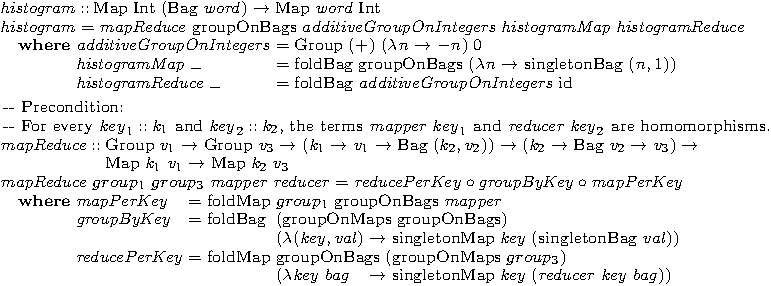
\includegraphics{pldi14/fig-mapReduce.pdf}
\caption{The $\Gl$-term $\HISTOGRAM$ with Haskell-like syntactic
  sugar. $\Term{additiveGroupOnIntegers}$ is the abelian group induced on
  integers by addition $(\mathbb{Z}, +, 0, -)$.}
\label{fig:case-study-pseudocode}
\end{figure*}

  
For base types with no known incrementalization strategy,
the precise interfaces for differentiation and
proof plugins can guide the implementation effort. These
interfaces could also from the basis for a library of
differentiation plugins that work well together.

Rewriting whole programs in our language would be an excessive
requirements. Instead, we embed our object language as an EDSL in
some more expressive meta-language (Scala in our case study), so
that embedded programs are reified. The embedded language can be
made to resemble the metalanguage~\citep{rompf2010lightweight}.
To incrementalize a part of a computation, we write it in our
embedded object language, invoke $\DERIVE$ on the embedded
program, optionally optimize the resulting programs and finally
invoke them. The metalanguage also acts as a macro system for the
object language, as usual. This allows us to simulate polymorphic
collections such as $\Bag*[\Gi]$ even though the object language is
simply-typed; technically, our plugin exposes a family of base
types to the object language.

\pg{Explain how we construct changes? The metalanguage can then
  construct changes in different ways?}



  \begin{oldSec}
\subsection{Methodology}
\label{ssec:methodology}


\begin{itemize}
\item We identify (classes of) base types which are relevant for
  our application, together with any relevant equational properties.
\item We define change representations for these base
  types.
\pg{Here we should give some criteria, if we can.}
\pg{For instance, restrictions on change structures which are
  erased become additional invariant for the change types.}
\pg{For instance, we should
  discuss the point of this paragraph:
``Furthermore, derivatives need to inspect the intensional
structure of changes, which are typically small, without applying
them to their base value, which is typically big. The interface
to do this depends on the specific change structure, hence we
specify no generic operation to allow this.''
}
\item We design for each (class of) base type a relevant set of
  primitives.  Where
  useful, we provide optimized derivatives for such primitives.
  We try to define primitives which capture
  incrementalizable computation skeletons; if such primitives are
  not general enough, we can add additional primitives which are
  more general but whose derivatives are less efficient.
\item We transform target programs to use our primitives.
\end{itemize}

\pg{I need self-maintainability and predicting nil changes here
  to discuss the example. So maybe the example should just be
  part of the case study.}
For instance, \citet{GlucheGrust97Incr} incrementalize bags for a
first-order language. By adapting/extending those techniques, we
can integrate bags into our higher-order language.

\pg{We should say dictionary, not map, for reduced ambiguity with the map operation.}
Using similar techniques, we also implemented support for the
operation on maps needed in our case study.

\pg{This section should also explain where changes come from.}
\end{oldSec}



\subsection{Predicting nil changes}
Handling changes to all inputs can induce excessive overhead in incremental
programs~\citep{Acar09}. It is also often
unnecessary; for instance, the function argument of $\Term{fold}$ in 
\cref{sec:intro} does not change since it is a closed subterm of the program, so
$\Term{fold}$ will receive a nil change for it.
A (conservative) static analysis can detect changes that are guaranteed to be nil at runtime. 
We can then specialize derivatives that receive this change, so that they need not
inspect the change at runtime.

For our case study, we have implemented a simple static analysis which
detects and propagates information about closed terms. The analysis is not interesting and 
we omit details for lack of space.



% Emacs, this is -*- latex -*-!

\subsection{Self-maintainability}
\label{sec:performance-cons}
\label{ssec:self-maint}

\begin{oldSec}
On its own, deriving $\Gl$-abstractions, applications and
variables (\cref{fig:correctness:derive}) does not improve performance.
It only relates the computations embodied in the primitives in
an incremental and higher-order setting, and provides a method to
generalize the vast quantity of research on first-order incremental
computation in the field of databases.
Our first approach toward performance gain is based on the idea of \emph{self-maintainable uses of primitives};
other approaches are certainly feasible. We did not formalize the
optimizations or prove them correct.
\end{oldSec}

In databases, a self-maintainable view~\citep{Gupta99MMV} is a function that can
update its result from input changes alone, without looking at
the actual input. By analogy, we call a derivative
\emph{self-maintainable} if it uses no
base parameters, only their changes. Self-maintainable derivatives
describe efficient incremental computations: since they do not
use their base input, their running time does not have to depend on the input
size.

\begin{examples}
$\Derive{\MERGE} = \Lam {x\; \D x\; y \; \D y}{\Merge{\D x}{\D y}}$
is self-maintainable with the
change structure $\ChangeStruct{\Bag{S}}$ described in
\cref{ssec:change-structures}, because it does not use the base
inputs $x$ and $y$.
Other derivatives are self-maintainable only in certain contexts.
The derivative of element-wise function application
$\App*{\App\MAP f}{\mathit{xs}}$ ignores the original
value of the bag $\mathit{xs}$ if the changes to
%
$f$ are always nil, because the underlying primitive $\FOLDBAG$
is self-maintainable in this case (as discussed in next section).
%
We take advantage of this by implementing a specialized
derivative for $\FOLDBAG$.

We have seen in \cref{ssec:differentiation} that $\Derivative$
needlessly recomputes $\Merge\Xs\Ys$. However, the result is a
base input to $\FOLD'$.
%
In next section, we'll replace $\FOLD'$ by a self-maintainable
derivative (based again on $\FOLDBAG$) and will avoid this
recomputation.
\end{examples}

%% Rationale for previous statement. Too complicated; left out.
%deriving a closed term without primitives yields a term that is
%self-maintainable whenever its higher-order arguments receive
%self-maintainable changes.
%The default rule $\Derive{c} = \Diff c c$ does not yield
%self-maintainable derivatives, because $\DIFF$ and $\APPLY$ use
%the input~$x$ in a significant way (\cref{fig:diff-apply}).
%However,

To conservatively predict whether a derivative is going to be
self-maintainable (and thus efficient), one can inspect whether
the program restricts itself to (conditionally) self-maintainable
primitives, like $\MERGE$ (always) or $\MAP \APP f$ (only if $\D
f$ is nil, which is guaranteed when $f$ is a closed term).

%% From the author response.
%It is possible to give a conservative approximation of whether a program's derivative is self-maintainable:
%If the original program only uses primitives with fully
%self-maintainable derivatives, the derivative of the program will
%be self-maintainable, too. We can syntactically approximate full
%self-maintainability of a primitive by checking whether the code
%of its derivative uses the $x$ variable (in addition to $\D x$) \pg{bind x! What about multiple arguments?}. For
%instance, the derivative of $\MERGE$ uses only $\D x$ and $\D y$, never $x$
%or $y$, and is hence fully self-maintainable. The derivative of
%$\FOLDBAG$ uses both $f$ and $\D f$; it is only self-maintainable
%sometimes (when df is the nil change).

\begin{oldSec}
Sometimes we can safely replace the derivative of a primitive by
a self-maintainable term, in which case we call it a
\emph{self-maintainable use of a primitive.}
Terms have self-maintainable derivatives if they use
primitives in a self-maintainable manner.

\pg{As Klaus points out, this is not true until we fix the set of
  changes - discussed in \#265. So we should specify the set of
  changes, or use a different example. We should also motivate
  it.}
%
\pg{Agreed: Convert to bags and to our running example, using foldBag.}
To illustrate, suppose $\MAP$ is a primitive of sets of
integers,
and changes to sets consist of insertions and deletions only.
The term
\[
\Lam x {\MapT {\Lam*n {n + 1}} x}
\]
contains a self-maintainable use of $\MAP$, because any change to
the input set~$x$, say $\{\App\INSERT5, \App\DELETE7\}$, can be
converted to an output change, say $\{\App\INSERT6,
\App\DELETE8\}$, without looking at $x$ itself. The use of $\MAP$
in the following term is not self-maintainable:
\[
\Lam x {\MapT {\Lam*n {n + \Sum* x}} x}.
\]
Even one insertion to the input set~$x$ generates a sweeping
change over all elements of the output set that is impossible to
express in terms of insertions and deletions without knowledge of $x$.

\pg{Before this, show that some of our primitives are
  self-maintainable, and some are self-maintainable if some
  inputs are nil.}
Our prototype optimization framework proceeds in two steps.
\begin{enumerate}
\item A static analysis identifies when changes are guaranteed to be nil.
\item During the differentiation transformation, $\DERIVE$
selects an appropriate self-maintainable function whenever possible,
considering the results of the static analysis.
\end{enumerate}
Due to space constraint, we cannot go into details of those
steps.
%
\yc{link to code}
%
\end{oldSec}

To avoid recomputing base arguments for self-maintainable derivatives
(which never need them), we
currently employ lazy evaluation.  Since we could use standard techniques for dead-code
elimination~\citep{Appel97} instead, laziness is not central to our
approach.

A significant restriction is that not-self-maintainable derivatives can require expensive computations to supply their base
arguments, which can be expensive to compute. Since they are also
computed while running the base program, one could reuse the previously
computed value through memoization or extensions of static
caching (as discussed in \cref{ssec:staticmemo}). We leave implementing these optimizations for future work. As a consequence,
our current implementation delivers good results only if
most derivatives are self-maintainable.

\begin{oldSec} % ID=Appel97
\pg{Do not remove without universal agreement. I don't think the paper can avoid discussing this aspect. }
One important issue is left. In a call-by-value
implementation of lambda calculus, running the program
\[
\Derive{\App{s}{t}} = \App{\App{\Derive{s}}{t}}{\Derive{t}}
\]
computes $t$
again, even though it was computed in the base program, thus
leading to wasteful repeated computation.
However, we claim this is a simpler problem to solve.
Three possibilities arise:
\begin{enumerate}
\item $t$ is very cheap to compute (for instance, it is a
  literal), so the problem does not occur.
\item $t$ is passed to a function which does not use it, hence
  we can avoid computing it using separate optimization steps, by
  executing the derivative with a lazy semantics (as done in our
  benchmarks) or (we expect) by using known techniques for
  interprocedural dead-code elimination~\citep{Appel97}.
\item Otherwise, since the term $t$
  was already computed while running the base
  program, we can save its value for use in the derivative.
  Approaches to
  implement this include memoization~\pg{cite} and extensions of
  static caching (as discussed in Sec.~\ref{sec:rw}).
  We leave investigating the different
  approaches to future work.
\end{enumerate}
\end{oldSec}

\begin{oldSec} % ID=Gupta99MMV
We next analyze when $t$ is going to be unused.
Inspecting the definition of $\DERIVE$ shows that only derivatives of (functions
containing) primitives can use $t$. For instance,
$\Derive{\Lam{x}{x}} = \Lam{x}{\Lam{\D x}{\D x}}$ does not use its
base input $x$, because $\Derive{x} = \D x$.
\pg{Make this more tentative. Remove 'prove'.}
It's easy to prove
by induction that if derivatives of primitives appearing in $s$
do not use their base input, neither does $s$.\footnote{Function
  changes coming from outside the program are not covered by this
  proof and are possible counterexamples.}

We term primitives whose derivative does not use their base input
self-maintainable, by analogy with the database concept of
self-maintainable views~\citep{Gupta99MMV}. \ko{Give example of 
self-maintainable and non-self-maintainable primitive}. 
We then extend this to programs: a
closed program is self-maintainable if its result does not depend
on base inputs or base intermediate results.
%
For programs which do not depend on functions as parameters (and
whose derivatives hence do not have function changes as
parameters), it should be straightforward to prove that being
self-maintainable is equivalent to only using self-maintainable
primitives.

Hence, we can argue informally that if a program only uses
self-maintainable primitives, its derivative will not recompute
base intermediate results (except if they are computed for
unrelated reasons). In our case study (Sec.~\ref{sec:eval}),
such derivatives are already
extremely efficient.

\pg{This should be somehow better integrated in the rest of the section.}
\end{oldSec}


\subsection{Case study}
\label{sec:plugins}


We perform a case study on a nontrivial realistic program to
demonstrate that \ILC\ can speed it up.
We take the MapReduce-based skeleton of the
word-count example~\citep{Lammel07}. We define a
suitable differentiation plugin, adapt the program to use it and show
that incremental computation is faster than recomputation.
%
We designed and implemented the differentiation plugin 
following the requirements of the corresponding proof plugin,
even though we did not formalize
the proof plugin (e.g. in Agda).
For lack of space, we focus on base types
which are crucial for our example and its performance, that is,
collections.
%
The plugin also implements tuples, tagged unions, Booleans and
integers with the usual introduction and elimination forms, with
few optimizations for their derivatives.

$\WORDCOUNT$ takes a map
from document IDs to documents and produces a map
from words appearing in the input to the count of their
appearances, that is, a histogram:
\[
\HasType \WORDCOUNT {\Fun {\HashMap \DOCUMENTID \DOCUMENT} {\HashMap \WORD \Int}}
\]
For simplicity, instead of modeling strings, we model documents
as bags of words and document IDs as integers. Hence, what we implement is:
\[
\HasType \HISTOGRAM {\Fun {\HashMap \Int {\Bag*[a]}} {\HashMap a \Int}}
\]
We model words by integers ($a = Int$), but treat them parametrically.
Other than that, we adapt directly
\citeauthor{Lammel07}'s code to our language.
\pg{But it cannot accept all the same parameters... Ah, but it
  depends on which foldMap we call. OK.}
\Cref{fig:case-study-pseudocode} shows the $\Gl$-term
$\HISTOGRAM$.

% Emacs, this is -*- latex -*-!
\begin{figure}

\centering

\lstinputlisting[language=scala,
firstline=10,
escapechar=|,
literate=
{=>}{$\Rightarrow\,$}2
{>=}{$\ge\;$}2
{<-}{$\leftarrow\;$}2
{!=}{$\ne\;$}2
{Abelian-group-based}{\text{Abelian-group-based }}1
{<}{$<$}2
{bag1}{{bag$_1$}}4
{bag2}{{bag$_2$}}4
{value1}{{value$_1$}}6
{value2}{{value$_2$}}6
{dict1}{{dict$_1$}}5
{dict2}{{dict$_2$}}5
{v1}{{v$_1$}}2
{v2}{{v$_2$}}2
{???}{$\ldots$}3
]{pldi14/mapReduce.scala}
\caption[A Scala implementation of primitives for bags and maps]{A Scala implementation of primitives for bags and maps.
In the code, we call $\boxplus$, $\boxminus$ and $e$ respectively \emph{merge}, \emph{inverse}, and \emph{zero}.
We also omit the relatively standard primitives.\pg{Can we now move this code to an appendix, since we explain so much in text?}}
\label{fig:primitives}
\end{figure}


\pg{Why does 'target language' show up all of a sudden? Shouldn't
  we say that we generate Scala code for execution
  \textbf{elsewhere}? Right now, we say it in next section. Confusing.}
%
\Cref{fig:primitives} shows a simplified
Scala implementation of the primitives
used in \cref{fig:case-study-pseudocode}.
As bag primitives, we provide constructors and a fold operation,
following \citet{GlucheGrust97Incr}. The constructors for bags
are $\Empty$ (constructing the empty bag), $\SINGLETON$
(constructing a bag with one element), $\MERGE$ (constructing the
merge of two bags) and $\NEGATE$ ($\Negate{b}$ constructs a bag
with the same elements as $b$ but negated multiplicities); all but $\SINGLETON$ represent
abelian group operations.
%
Unlike for usual ADT constructors, the same bag can be
constructed in different ways, which are equivalent by the equations defining abelian groups;
for instance, since $\MERGE$ is commutative, $\Merge{x}{y} = \Merge{y}{x}$.
%
Folding on a bag will represent the bag through constructors in
an arbitrary way, and then replace constructors with arguments;
to ensure a well-defined result, the arguments of fold should
respect the same equations, that is, they should form an abelian group;
for instance, the binary operator should be commutative.
%
Hence, the fold operator $\FOLDBAG$ can be defined to take a
function (corresponding to $\SINGLETON$) and an abelian group
(for the other constructors). $\FOLDBAG$ is then defined by equations:
%
\begin{alignat*}{2}
&  \HasType{\FOLDBAG}{\mathbf{Group}\; \Gt \to (\Gs \to \Gt) \to &&\Bag[\Gs] \to \Gt}\\
&  \App{\FoldBag {g @ (\_, \boxplus, \boxminus, e)}{f}}{\Empty}
    &&= e \displaybreak[0]\\
&  \App{\FoldBag {g @ (\_, \boxplus, \boxminus, e)}{f}}{\Merge* {b_1} {b_2}}
   &&= \App{\FoldBag{g}{f}}{b_1} \displaybreak[0]\\
&&& \boxplus
  \App{\FoldBag{g}{f}}{b_1} \displaybreak[0]\\
&  \App{\FoldBag {g @ (\_, \boxplus, \boxminus, e)}{f}}{\Negate* b}
   && = \boxminus \; \App*{\FoldBag{g}{f}}{b}\displaybreak[0]\\
&  \App{\FoldBag {g @ (\_, \boxplus, \boxminus, e)}{f}}{\Singleton*{v}}
   &&= \App{f}{v}
\end{alignat*}
%
If $g$ is a group,
these equations specify $\App{\FOLDBAG} g$ precisely~\citep{GlucheGrust97Incr}.
%
Moreover, the first three equations mean that $\FoldBag{g}{f}$ is \emph{abelian group
  homomorphism} between the abelian group on bags and the group
$g$ (because those equations coincide with the definition).
%
\Cref{fig:primitives} shows an implementation of $\FOLDBAG$ as
specified above.
Moreover, all functions which deconstruct a bag can be expressed in
terms of $\FOLDBAG$ with suitable arguments.
%
For instance, we can sum the elements of a bag of integers with
$\FoldBag{\Term{gZ}}{\Lam*{x}{x}}$, where
$\Term{gZ}$ is the abelian group on integers defined in
\cref{ssec:change-structures}.
Users of $\FOLDBAG$ can define different abelian groups to specify
different operations (for instance, to multiply floating-point numbers).

If $g$ and $f$ do not change, $\FoldBag{g}{f}$ has a self-maintainable
derivative.
By the equations above,
\pg{Non-standard alignment, because the last line doesn't fit.}
\begin{align*}
& \FoldBag{g}{f} \Update*{b}{\D b}\displaybreak[0]\\
=\;& \FoldBag{g}{f} {(\Merge b {\D b})}\\
=\;& \App{\FoldBag{g}{f}}{b}  \boxplus \App{\FoldBag{g}{f}}{\D b} \\
=\;& \Update{\App{\FoldBag{g}{f}}{b}}{\Term{GroupChange} \; g \; \left(\App{\FoldBag{g}{f}}{\D b}\right)}
\end{align*}
We will describe the $\Term{GroupChange}$ change constructor in a moment.
Before that, we note that as a consequence, the derivative of $\FoldBag{g}{f} $ is
\[
\Lam{b \; db} \Term{GroupChange} \; g \; \left(\App{\FoldBag{g}{f}}{\D b}\right)\text{,}
\]
and we can see it does not use $b$: as desired, it is
\emph{self-maintainable}. Additional restrictions are require to
make $\FOLDMAP$'s derivative self-maintainable. Those restrictions require the
precondition on $\Term{mapReduce}$ in
\cref{fig:case-study-pseudocode}. $\Term{foldMapGen}$ has the
same implementation but without those restrictions; as a
consequence, its derivative is not self-maintainable, but it is more generally applicable.
Lack of space prevents us from giving more details.

To define $\Term{GroupChange}$, we need a suitable erased change
structure on $\Gt$, such that $\UPDATE$ will be equivalent to
$\boxplus$. Since there might be multiple groups on $\Gt$, we
\emph{allow the changes to specify a group}, and have
$\UPDATE$ delegate to $\boxplus$:
\begin{align*}
& \Change{\Gt} = \Term{Replace}\; \Gt \mid \Term{GroupChange} \Abelian*{\Gt} \Gt \\
& \Update{v}{(\Term{Replace} \; u)} = u\\
& \Update{v}{(\Term{GroupChange} \; (\bullet, \Term{inverse}, \Term{zero})\; dv)} = v \bullet dv\\
& \Diff{v}{u} = \Term{Replace}\; v
\end{align*}
That is, a change between two values is either simply the new
value (which replaces the old one, triggering recomputation),
or their difference (computed with abelian group
operations, like in the changes structures for groups from
\cref{ssec:change-structures}. The operator $\DIFF$
does not know which group to use, so it does not take advantage
of the group structure.
However, $\FOLDBAG$ is now able to generate a group change.
% Rewrite:
%derivatives of primitives like $\FOLDBAG$ can
%use the group structure they have available when producing changes.
%
\pg{Clarify about user-defined groups.}

We rewrite $\Program$ in terms of $\FOLDBAG$ to take advantage of
group-based changes.
{\DeriveProgramEnv
\begin{align*}
&\Term{id}=\Lam{x}{x}\\
&G_+ = (\mathbb Z, +, -, 0)\\
&\Program = \Lam{\Xs}{\Lam{\Ys}{\FOLDBAG~G_+~\Term{id}~(\Merge\Xs\Ys)}}\\
&\Derive\Program=\\
&\zero
\Lam{\Xs}{\Lam{\DXs}{}}\Lam{\Ys}{\Lam{\DYs}{}}\\
&\one
\FOLDBAG'~G_+~G_+'~\Term{id}~\Term{id}'\\
&\two
(\Merge\Xs\Ys)\\
&\two
(\MERGE'~\Xs~\DXs~\Ys~\DYs)
\end{align*}
}%
It is now possible to write down the derivative of $\FOLDBAG$.
{\DeriveProgramEnv
\begin{align*}
&\text{(if static analysis detects that $\D G$ and $\D f$
are nil changes)}\\
&\FOLDBAG'=\Derive{\FOLDBAG}=\\
&\zero
\Lam{G}{\Lam{\D G}{\Lam{f}{\Lam{\D f}{
\Lam{\Zs}{\Lam{\DZs}{}}}}}}\\
&\one
\Term{GroupChange}~G~
(\FOLDBAG~G~f~\DZs)
\end{align*}
}%
We know from \cref{ssec:plugin} that
\[
\MERGE'=\Lam{u}{\Lam{\D u}{\Lam{v}{\Lam{\D v}{\Merge{\D u}{\D v}}}}}.
\]
Inlining $\FOLDBAG'$ and $\MERGE'$ gives us a more readable term
$\beta$-equivalent to the derivative of $\Program$:
{\DeriveProgramEnv
\begin{align*}
&\Derive\Program=\\
&\zero
\Lam{\Xs}{\Lam{\DXs}{}}\Lam{\Ys}{\Lam{\DYs}{}}
%
\FOLDBAG~G_+~\Term{id}~
(\MERGE~\DXs~\DYs).
\end{align*}
}%

\begin{oldSec}
Function destructing bags must be homomorphisms between abelian
groups~\citep{GlucheGrust97Incr}, and can all be defined in terms
of $\FOLDBAG$. More in general, bags form an abelian
\emph{collection group}.
%
%To incrementalize bags, we reuse the change structure on bags
%described in \cref{ssec:change-structures}.
%
An abelian group on $\Gi$ can be lifted to an abelian collection
group on $(\HashMap{\kappa}{\Gi})$ through \emph{mapGroup}, so that we
can apply similar ideas to maps. The resulting primitives for map
are expressive enough to efficiently incrementalize our example
program.

Destructing an abelian collection group produces a value in an
abelian group (such as integers or abelian collection groups). To
avoid hardcoding which group to use, we define a general change
structure for abelian groups. After erasure, the change structure is as follows
(cf.~\cref{fig:change-operations,fig:case-study-pseudocode}):\footnote{For clarity, we use ADTs and pattern matching instead of sum types.}
...

The derivative of $\App{\FOLDBAG}{f}$ is efficient on $\Term{Update}$ changes when $df$ is
known to be a nil change; in that case,
$\App{\FOLDBAG}{f}$ is a homomorphism, hence self-maintainable (\cref{sec:performance-cons}). To see why, take any homomorphism $\HasType f {\Fun \Gs \Gt}$ 
between user-defined
abelian groups $G_\Gs$ and $G_\Gt$, and suppose
$\D v = \HasType{\Term{Update} \; (G_\Gs, u)}{\Change \Gs}$. By homomorphism properties,
\begin{align*}
\App f {\Update*{v}{\D v}}
&= \App f {(v \bullet_\Gs u)}
= \App* f v  \bullet_\Gt \App* f u \\
&= \Update{\App* f v}{\Term{Update} \;(G_\Gt, \App f u)}.
\end{align*}
The derivative of $f$ on
$\Term{Update}$ changes is then $\App{\App{f'}{v}}{(\Term{Update} \; (G_\Gs, u))} = \Term{Update} \; (G_\Gt, \App f u)$,
by \cref{def:derivatives}.
$f'$
requires no information about $v$, therefore it is
self-maintainable. That is the
principle behind all derivatives in the plugin that are faster
than recomputation.
\end{oldSec}

\begin{oldSec}
\subsubsection{Bags}

We apply \citeauthor{GlucheGrust97Incr}'s approach to view
maintenance based on monoid- and group-homomorphisms
\citep{GlucheGrust97Incr}. An operation $f$ on a collection is
effectively incrementalized if the collection type forms a group
$G$, and $f$ is a homomorphism from $G$ to some group over its
result type. Bags with signed multiplicities%
%
\footnote{Bags with signed multiplicities correspond to databases
described in \citet{Koch10IQE}, where tuples are allowed to have
negative multiplicities. Bag elements with negative
multiplicities represent deletion of themselves.}
%
form the free abelian group over their element type; their nice
properties are particularly suitable for our purposes.
Incremental computation based on noncommutative groups requires
caching intermediate results, and we leave it for future work.

Bag constructors $\Empty$, $\SINGLETON$, $\MERGE$ are identical
to those used in \citet{GlucheGrust97Incr}. We add a primitive
$\NEGATE$ to create bags with negative multiplicities.
% listing order follows argument order of $\FOLDBAG$.
\begin{align*}
\HasTypeAligned{\MERGE}
  {\Fun{\Fun{\Bag[\Gi]}{\Bag[\Gi]}}{\Bag[\Gi]}}
\\
\HasTypeAligned{\NEGATE}
  {\Fun{\Gi}{\Bag[\Gi]}}
\\
\HasTypeAligned{\Empty}
  {\Bag[\Gi]}
\\
\HasTypeAligned{\SINGLETON}
  {\Fun{\Gi}{\Bag[\Gi]}}
\end{align*}
If we consider $\NEGATE$ to be another bag constructor, then a
natural elimination form of bags is the primitive $\FOLDBAG$:
\begin{align*}
\HasTypeAligned\FOLDBAG
  {\Fun {\Abelian \Gi}
    {\Fun {\Fun*{\Gi}{\Gt}} {\Gt}}}
\\
\Abelian\Gi
  & =      \Fun*{\Base\Gi}{\Fun{\Base\Gi}{\Base\Gi}} \\
  & \times \Fun*{\Base\Gi}{\Base\Gi} \\
  & \times \Base*\Gi.
\end{align*}
\citet{GlucheGrust97Incr} implement many object query language
views in terms of $\FOLDBAG$ to show that they are
homomorphisms and easily incrementalized. Since our framework
supports higher-order functions, we can actually offer
$\FOLDBAG$ to users, who are then free to write all kinds of
easily incrementalized homomorphisms
(\cref{foldBag-homomorphism}).

% Actually, the fact & lemma below talk about functions in the
% semantic domain. Semantic brackets are left out by abusing
% notation.
\begin{definition}[Semantics of bag primitives]~
\begin{subdefinition}
\item $\Eval{\Bag[\Gi]}$ is the free abelian group with basis $\Eval\Gi$.
\item $\MERGE$ evaluates to the binary operator of the free abelian
group.
\item $\NEGATE$ evaluates to the function that takes every
element of $\Eval{\Bag[\Gi]}$ to its inverse in the free abelian
group.
\item $\Empty$ evaluates to the identity element of the free
abelian group.
\item\label{foldBag-homomorphism} If
$\HasType{G_\tau}{\Abelian\tau}$ evaluates to an abelian group,
then for every term $\HasType f {\Fun\Gi\Gt}$, the term
$\App*{\App\FOLDBAG{G_\tau}}{f}$ evaluates to the unique
homomorphism%
\footnote{ The universal property of free abelian groups
guarantees the existence and uniqueness of such a homomorphism. A
constructive proof of the universal property doubles as a
specification of $\FOLDBAG$. } %
from the free abelian group on $\Gi$ to the group denoted by
$G_\tau$.
\end{subdefinition}
\end{definition}

\subsubsection{Maps}

There is no obvious abelian group structure on maps as there is
on bags. However, $\HashMap\Gk\Gi$ can be thought of as (possibly
infinite) vectors over nullable values of type $\Gi$ indexed by
all values of type $\Gk$. It suggests the group structure on maps
as an indexed direct product of a group structure on $\Gi$. The
formulation would be more elegant if there were dependent type
support in the object language.

These are the primitives on maps.
\begin{align*}
\HasTypeAligned\MAKEMAP
  {\Fun\Gk{\Fun\Gi{\HashMap\Gk\Gi}}}
\\
\HasTypeAligned\LOOKUP
  {\Fun\Gk{\Fun{\Map\Gk\Gi}{\Maybe\Gi}}}
\\
\HasTypeAligned\LIFTGROUP
  \Fun{\Abelian\Gi}{\Abelian{\HashMap\Gk\Gi}}
\\
\HasTypeAligned\FOLDMAP
  \Fun{\Abelian\Gi}
    {\Fun{\Abelian\Gt} \\ & \qquad
      {\Fun{ \Fun*\Gk{\Fun\Gi\Gt} }
        {\Fun{\HashMap\Gk\Gi} \Gt}}}
\end{align*}

\begin{definition}[Semantics of map primitives]~
\begin{subdefinition}
\item $\Eval{\Map\Gk\Gi}$ is the set of partial functions from
$\Eval\Gk$ to $\Eval\Gi$ defined only at a finite number of
points.
\item $\MAKEMAP$ evaluates to the function that converts a
key-value pair to the corresponding partial function defined at
1 point.
\item $\LOOKUP$ evaluates to the standard lookup function on
maps.
\item $\LIFTGROUP$ evaluates to a function that maps abelian
groups $G_\Gi$ over $\Eval\Gi$ to the abelian group formed by
direct product of copies of $G_\Gi$ indexed by $\Eval\Gk$. Its
identity element, binary operation and inverse function are the
empty map, map merge and map negation.
\item Given a map $\HasType m {\HashMap\Gk\Gi}$, abelian groups
$G_\Gi$, $G_\Gt$, and a function $\HasType f
{\Fun\Gk{\Fun\Gi\Gt}}$ such that $\App*fk$ is a homomorphism from
$G_\Gi$ to $G_\Gt$ for every $\HasType k\Gk$, the term
\[
\App{\App{\App{\App\FOLDMAP{G_\Gi}}{G_\Gt}}f}m
\]
evaluates to a value in $\Eval\Gt$ by the following steps (we
write $m(k)$ for the value of the map $m$ at key $k$).
\begin{enumerate}
\item Replace each $m(k)$ by $\App*{\App fk}{m(k)}$ to create the
map $\HasType{m'}{\HashMap\Gk\Gt}$.
\item Sum all values of $m'$ by the binary operation of $G_\Gt$.
\end{enumerate}
Since both steps are homomorphisms,
$\App*{\App{\App\FOLDMAP{G_\Gi}}{G_\Gt}}f$ is a homomorphism
from $\App*\LIFTGROUP{G_\Gi}$ to $G_\Gt$.
% to the unique homomorphism%
% \footnote{The existence and uniqueness of such a homomorphism is
% guaranteed by the universal property of indexed direct product
% as a product in the category of abelian groups.} %
% from $\App*\LIFTGROUP{G_\Gi}$ to $G_\Gt$ that agrees with
% $\App*fk$ for every $\HasType k \Gk$.
%
\end{subdefinition}
\end{definition}

Since our object language lacks dependent types, the user has to
make sure that the higher-order argument of $\FOLDMAP$ gives
rise to homomorphisms. This is the price paid for the
expressivity of user-defined groups.

\end{oldSec}
% Below are previous formulations.

% OLDSEC: rephrased skeleton & pointers
\begin{oldSec}
We perform a case study applying our technique to a MapReduce
skeleton. To this end, we implemented in Scala a language plugin
supporting some collections. We restricted ourselves to
primitives whose derivatives could be made self-maintainable.

To this end, we recast and extend some ideas by
\citet{GlucheGrust97Incr} and \citet{Koch10IQE} in our framework.
The collections we consider are maps and bags with negative
multiplicities. We use negative multiplicites to represent
removal of elements.%
%
\footnote{Our framework allows having standard bags as base types
  and bags with negative multiplicities as their change type. We
  leave this and a few other extension for future work.}
%
Bag elements must be comparable for equality, and this excludes
functions. Moreover, storing functions in data is hard because
the derivative of code extracting and using the function must
also have access to the derivative of that function. We plan to
augment base programs to also store function derivatives together
with the functions, but leave this for future work. \pg{Say
  something more.}

\pg{Write instantiation for bags.}
\begin{figure}[h]
\begin{align*}
\Change[\Bag \iota]{b} & = \Bag \iota\\
\Diff[\Bag \iota]{x}{y} & = \Merge x {\Negate*y}\\[\eqsep]
\Apply[\Bag \iota]{\D x}{x} & = \Merge x y
\end{align*}
%\caption{Term difference and change application.}
%\label{fig:plug-diff-apply}
\end{figure}
\end{oldSec}

% OLDSEC: skeleton.
% Refer for ideas.
\begin{oldSec}
We will illustrate a fully instantiated differentiation framework
by the simplest plugin expressive enough for nontrivial
applications. We will not prove the properties required of the
plugin for correctness to hold, but we believe that they are
true.

We designed the plugin around abelian groups.
Abelian groups are good for incrementalizing folds over a
collection because the irrelevance of folding order and the
possibility of removing an element from the fold via its inverse
means that we don't have to save any intermediate result. We
shall not investigate the caching aspect of incrementalization;
we do it later.

Some base types have changes based on abelian groups. Other base
types (sums) don't, but are still useful. Our plugin does not
make everything efficient. We give some primitives fast
derivatives now, and plan to support more and more primitives to
allow more and more fast derivatives.

By the way, we forbid functions in collections because nil
changes to functions have computation content and can't be
discarded. [Illustrating example: Klaus's f]

\subsection*{Details}

Listing: base types, their change types, DIFF, UPDATE

Those fall into 2 categories: those whose change we don't care
about (simply use replacement), and those whose change we care
about (change is either replacement value, or user-supplied
abelian group together with a group element.

Listing: derivatives

We can talk about foldBag and foldMap alone, leaving
everything else the difference with itself (that is, stupid
derivative by recomputation).
\end{oldSec}

% OLDSEC: abelian groups
% Refer to it when discussing AbelianDerivation traits.
\begin{oldSec}
Our approach is parametric in the concrete representation of
changes of type $\Change{\tau}$ as long as changes support the
operations listed in \cref{fig:change-operations}).
The update operator $\Apply{\D x}{x}$ updates a value $x$ with a
change $\D x$. The difference operator $\Diff{y}{x}$ computes the
change from $x$ to $y$.
And the nil change operator $\Nil{x}$
denotes the change that updates the value $x$ into itself.

In fact, if $\tau$ forms a group $\langle \tau, 0, +, -\rangle$,
we can define $\Diff{v_2}{v_1} = v_2 + (- v_1)$; for some groups,
we can use the resulting definition for incremental computation
\pg{not clear what this means yet}, as we will see later.
However, many interesting datatypes do not form groups, such as
functions or lists (\citet{GlucheGrust97Incr} introduce a group
structure for lists, but it is too restrictive\pg{elaborate});
hence we introduce here a more general abstraction, which can be
implemented via groups \pg{reorder this with the previous
  paragraph}.

\pg{I write $\cdot-\cdot$ for a binary operation, but I need something better.}
For instance, we can take $\tau$ to be the set of integers $\bz$. Integers are
the support of the commutative group $(\bz, \cdot + \cdot, 0, -\cdot)$, hence they are equipped
with a difference operation $\cdot-\cdot = \Gl x y. x + (-y)$. We can thus represent
changes for relative numbers with relative numbers: $\Diff{v_2}{v_1} = v_2 -
v_1$.

More formally, take an arbitrary type $\tau$ and values $v_1, v_2$ of
these type. We can describe the difference between these two values
with $\D v = \Diff{v_2}{v_1}$: this evaluates to a change $\D v$ which is
valid for $v_1$. Moreover, we can apply \pg{is this the term to use?} this change to a value
with $\Apply{\D v}v$. We have the guarantee that
$\Apply{\left(\Diff{v_2}{v_1}\right)}{v_1} = v_2$. In general, if we
apply changes to values for which they are not valid, our axioms do
not specify the result. Moreover, our axioms for arbitrary base types
only guarantee that a change $\Diff{v_2}{v_1}$ is valid for $v_1$,
even though, for many implementations of changes, $\Diff{v_2}{v_1}$ is
valid for values other than $v_1$. This is the case in particular if
the base type forms a group and we define changes reusing this group
structure, as we did for integers. In interesting applications, however, changes
are not generated directly by $\DIFF$.

Moreover, if $\D v$ is a valid change, we also have
$\Diff{\left(\Apply{\D v}v\right)}v = \D v$.

Our presentation of the behavior of changes on a datatype forms
an algebraic specification (excluding the concept of validity and
the properties which only apply to valid changes). In particular,
we can define a signature having sorts $\tau$ and $\Change{\tau}$,
the functions from \cref{fig:change-operations}
and equations (or axioms):
\begin{align*}
\Apply{\Diff*{s₂}{s₁}}{s₁} &= s₂\\
\Apply{\Nil{s}}{s} &= s\\
\end{align*}
\pg{Check which ones we have already proven.}

Since this set of axioms is algebraic (that is, purely first
order), we know from universal algebra~\citep{Mitchell1996foundations} that equational reasoning
is sound and complete for all models (implementations) of this
algebraic specification.

Moreover, we can show that those axioms are consistent by
providing models implementing them. \pg{Resume}
%Additionally, we have two implementations of those axioms.
\pg{A couple more axioms need to be checked.}
%
% (s₂ ⊝ (ds ⊕ s₁)) ∘ ds &= s₂ ⊝ s₁ (?)
%
% Special case:
%	(ds ⊕ s) ⊝ s = ds (EDIT: only if ds is valid for s).
%
% Therorems:
%
%s ⊝ s = nil s
%(s₁ ⊝ s₂) ∘ (s₂ ⊝ s₃) = s₁ ⊝ s₃
\end{oldSec}

\subsection{Benchmark results}

Our results show (\cref{fig:graph}) that our program reacts to input changes
in essentially constant time, as expected, hence orders of magnitude faster than
recomputation. Constant factors are small enough that the speedup is apparent on realistic input sizes.

For lack of space, details on benchmarking results and inputs
are available in the extended version of our paper (Appendix A).

Two important lessons from the evaluations are:
\begin{itemize}
\item As anticipated in \cref{ssec:self-maint}, to achieve good performance our current
  implementation requires some form of dead code elimination, such as laziness.
%Either laziness or dead-code elimination is required for
%good performance ().
\item Incrementalization increases code size significantly.
  Analyzing and addressing this increase is left for future work.
\end{itemize}

\begin{figure}
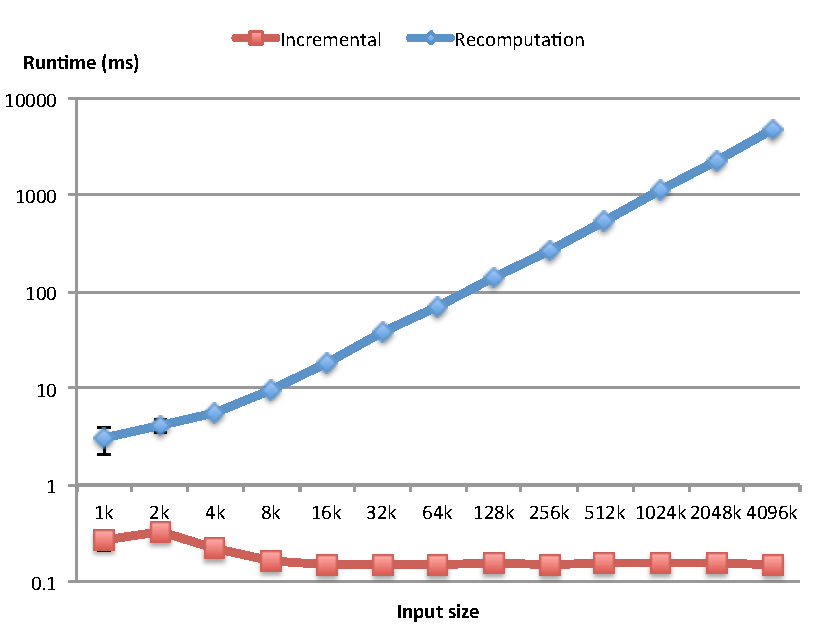
\includegraphics[keepaspectratio,width=8.5cm]{pldi14/HistogramGenerated-new.pdf}
\caption{Performance results in log-log scale, with input size on
  the x-axis and runtime in ms on the y-axis. Confidence
  intervals are shown by the whiskers; most whiskers are
  too small to be visible.}
\label{fig:graph}
\end{figure}


% Emacs, this is -*- latex -*-!
\chapter{Related work}
\label{sec:rw}

Existing work on incremental computation can be divided into two
groups: Static incrementalization and dynamic incrementalization.
Static approaches analyze a program statically and generate an incremental
version of it. Dynamic approaches create dynamic dependency graphs while
the program runs and propagate changes along these graphs.

The trade-off between the two is that static approaches have the potential
to be faster because no dependency tracking at runtime is needed, whereas
dynamic approaches can support more expressive programming languages.
%
\ILC\ is a static approach, but compared to the other static
approaches it supports more expressive languages.

In the remainder of this section, we analyze the relation to the
most closely related prior works. \Citet{Ramalingam93}, \citet{Gupta99MMV}
and \citet{Acar06} discuss further related work.


\section{Dynamic approaches}
One of the most advanced dynamic approach to incrementalization is
self-adjusting computation, which has been applied to Standard ML
and large subsets of C~\citep{Acar09,Hammer11}.
In this approach, programs execute on the original
input in an enhanced runtime environment that tracks the
dependencies between values in a \emph{dynamic
  dependence graph}~\citep{Acar06}; intermediate results are
memoized.
Later, changes to the input propagate through
dependency graphs from changed inputs to results,
updating both intermediate and final results;
this processing is often more efficient than recomputation.

However, creating dynamic
dependence graphs imposes a large constant-factor overhead during
runtime, ranging from 2 to 30 in reported
experiments~\citep{Acar09EAS,Acar10TDT}, and affecting the
initial run of the program on its base input.
\citet{Acar10TDT} show how to support high-level data
types in the context of self-adjusting computation; however, the
approach still requires expensive runtime bookkeeping during the initial run.
Our approach, like other static ones, uses a standard runtime
environment and has no overhead
during base computation, but may be less efficient when processing
changes. This pays off if the initial input is 
big compared to its changes.


\citet{Chen11} have developed a static transformation for purely
functional programs, but this transformation just provides a superior interface to use
the runtime support with less boilerplate, and does not reduce
this performance overhead. Hence, it is still a dynamic approach, unlike
the transformation this work presents.

Another property of self-adjusting computation
is that incrementalization is only efficient if the program has a suitable
computation structure. For instance, a program
folding the elements of a bag with a left or right fold will not
have efficient incremental behavior; instead, it's necessary that
the fold be shaped like a balanced tree. In general,
incremental computations become efficient only if they are \emph{stable}~\citep{Acar05}.
Hence one may need to massage the program to make it efficient. Our methodology is 
different: Since we do not aim to incrementalize arbitrary programs written in standard
programming languages, we can select primitives that have efficient derivatives and thereby require 
the programmer to use them.

Functional reactive programming \citep{Elliott:1997:FRA:258948.258973}
can also be seen as a dynamic approach to incremental computation;
recent work by \citet{Maier2013} has
focused on speeding up reactions to input changes by making them
incremental on collections. \citet{Willis08} use dynamic techniques
 to incrementalize JQL queries.

\section{Static approaches}
\pg{If we discuss partial evaluation, we should compare to
  \citep{Sundaresh91}}
Static approaches analyze a program at compile-time and produce an
incremental version that efficiently updates the output
of the original program according to changing inputs.

Static approaches have the potential to be more efficient than dynamic approaches,
because no bookkeeping at runtime is required. Also, the computed incremental
versions can often be optimized using standard compiler techniques
such as constant folding or inlining.
However, none of them support first-class functions; some
approaches have further restrictions.

Our aim is to apply static incrementalization to more expressive languages;
in particular, \ILC\ supports first-class functions and an open
set of base types with associated primitive operations.

\subsection{Finite differencing}
\label{sec:finite-diff}
\citet{Paige82FDC} present derivatives for a first-order language
with a fixed set of primitives.
\citet{Blakeley:1986:EUM} apply these ideas to a class of relational queries.
The database community extended
this work to queries on relational data, such as in \emph{algebraic
  differencing}~\citep{Gupta99MMV}, which inspired our work and
terminology. However, most of this work does not apply to nested
collections or algebraic data types, but only to relational
(flat) data, and no previous approach handles first-class
functions. Incremental support is typically designed
monolithically for a whole language, rather than piecewise.
Improving on algebraic differencing, \citet{Koch10IQE}
\emph{guarantees} asymptotic speedups with a compositional query
transformation and delivers huge speedup in realistic benchmarks,
though still for a first-order database language.
\pg{continue with new work, discuss why we don't do iterated differentiation.}

More general (non-relational) data types are considered in the work by \citet{GlucheGrust97Incr};
our support for bags and the use of groups is inspired by their work,
but their architecture is still rather restrictive: they lack
support for function changes and restrict incrementalization to
self-maintainable views, without hinting at a possible solution.

\subsection{Static memoization}
\label{ssec:staticmemo}
\citeauthor{Liu00}'s work~\citep{Liu00} allows to incrementalize a first-order base
program $f(\Old{x})$ to compute $f(\New{x})$, knowing how
$\New{x}$ is related to $\Old{x}$. To this end, they transform
$f(\New{x})$ into an incremental program which reuses the
intermediate results produced while computing $f(\Old{x})$, the
base program. To this end, (i) first the base program is
transformed to save all its intermediate results, then (ii) the
incremental program is transformed to reuse those intermediate
results, and finally (iii) intermediate results which are not
needed are pruned from the base program. However, to reuse
intermediate results, the incremental program must often be
rearranged, using some form of equational reasoning, into some
equivalent program where partial results appear literally. For
instance, if the base program $f$ uses a left fold to sum the
elements of a list of integers $\Old{x}$, accessing them from the
head onwards, and $\New{x}$ prepends a new element $h$ to the
list, at no point does $f(\New{x})$ recompute the same results.
But since addition is commutative on integers, we can rewrite
$f(\New{x})$ as $f(\Old{x}) + h$. The author's CACHET system will
try to perform such rewritings automatically, but it is not
guaranteed to succeed. Similarly, CACHET will try to synthesize
any additional results which can be computed cheaply by the base
program to help make the incremental program more efficient.

Since it is hard to fully automate such reasoning, we move
equational reasoning to the plugin design phase. A 
plugin provides general-purpose higher-order primitives for which
the plugin authors have devised efficient derivatives (by using
equational reasoning in the design phase). Then, the
differentiation algorithm computes incremental
versions of user programs without requiring further user intervention.
It would be useful to combine \ILC\ with some form of static
caching to make the computation of derivatives which
are not self-maintainable more efficient. We plan to do so
in future work.
%Our approach is instead fully automatic, and will always produce
%a result, which in the worst case will merely be slow;
%% they can also fail and then 'produce a slow program'.
%
%we envision the use of directed rewrite rules for further
%optimization of programs, instead of undirected search.
%% Not so important.

\chapter{Conclusion}
\label{ssec:future}
In this part we have presented \ILC, an approach to lifting incremental computations
on first-order programs to incremental computations on higher-order
programs. We have presented a machine-checked correctness proof 
of a formalization of \ILC\ and an initial experimental evaluation
in the form of an implementation, a sample plugin for maps and bags,
and a non-trivial example that was incrementalized successfully and
efficiently. 

\pg{Revise}
Our work opens several avenues of future work. Our current implementation
is not efficient on derivatives that are not self-maintainable.
However, as discussed
(Sec.~\ref{ssec:self-maint}), we will study how
to memoize intermediate results to address this limitation. Our next
step will be to develop language plugins which
have efficient non-self-maintainable primitives.

Another area of future work is adding support for algebraic data
types (including recursive types), polymorphism, subtyping, general recursion
and other collection types. While support for algebraic data
types could subsume support for specific collections, many
collections have additional algebraic properties that enable faster
incrementalization (like bags). Even lists (which have fewer algebraic properties)
can benefit from special support~\citep{Maier2013}.

Moreover, we intend to apply \ILC{} to optimize queries on
collections in the context of the \textsc{SQuOpt}
project~\citep{GiarrussoAOSD13}, which was a motivation for this
work; in particular, \textsc{SQuOpt} can automatically rewrite
queries to use database-style indexes, and \ILC{} enables
updating those indexes when input data changes.

\begin{oldSec}
Our derivatives accept arbitrary changes for all inputs. We plan
to stage the code that updates the inputs through lightweight
modular staging~\citep{rompf2010lightweight}, analyze it to
predict changes and specialize the derivative to the result of
this analysis. For instance, if we need to update $\Term{f} \;
\Term{bag}$ after $\Term{bagNew} = \Term{insert} \; \Term{el} \;
\Term{bagOld}$, we can infer that $\Term{dbag}$ is an insertion
and specialize $f'$ to such a change.
\end{oldSec}

Finally, we intend to perform a full and thorough experimental evaluation
to demonstrate that \ILC\ can incrementalize large-scale practical programs.


% Temporarily omitted as part of the double-blind review process.
\iftoggle{names}{
\acks
% Emacs, this is -*- latex -*-!

\chapter*{Acknowledgments}
\phantomsection
\addcontentsline{toc}{chapter}{Acknowledgments}
% From AOSD13
I thank Sebastian Erdweg for helpful discussions on
this project, Katharina Haselhorst for help
implementing the code generator, and the anonymous reviewers, Jacques Carette and Karl Klose
for their helpful comments on this chapter.
This work is supported in part by the European Research Council, grant \#203099 ``ScalPL''.

% From PLDI14 (?)
% From ILC17
We thank Cai Yufei, Tillmann Rendel, Lourdes Del Carmen Gonz\`alez Huesca, Yann
R\`egis-Gianas, Philipp Schuster, Sebastian Erdweg, Marc Lasson, Robert Atkey,
... for helpful discussions on this project.
}{}

\bibliographystyle{abbrvnat}

% The bibliography should be embedded for camera-ready submission, not
% for now.

\bibliography{../../Bibs/ProgLang,../../Bibs/DB,../../Bibs/own,../../Bibs/SoftEng}

\appendix
\begin{oldSec}
% Emacs, this is -*- latex -*-!
\section{Correctness proof of derivation on simply typed lambda
  terms}
\label{sec:STLC-correct}

\yc{claim correspondence to Agda script}
\pg{Lots of this should move to earlier in the paper, and should not be repeated here. Remember to update this section.}
Let $\GD\Gs$ be the type of changes to values of type $\Gs$. Let
us specify $\GD\Gs$ recursively thus:
\begin{align*}
\GD(\Gs\r\Gt)&=\Gs \r \GD\Gs \r \GD\Gt,\\
\GD\Gi&=\Gi.
\end{align*}
Intuitively, the change to a function is a function computing
changes on the result values, and the change to an individual is
its replacement.
We chose the type of changes $\GD\Gi$ to an individual for
simplicity of presentation; its triviality does not hide the
technical issues associated with derivatives.

As seen before \yc{link to justification},
the derivative of a function of type $(\Gs\r\Gt)$ has the type
$\GD(\Gs\r\Gt)=\Gs\r\GD\Gs\r\GD\Gt$.
Let $\Derive{\cdot}$ be the program transformation that produces
derivatives from terms. Below is the most obvious
\pg{I do not like ``obvious'' here} type-correct
implementation.
\begin{align*}
\Derive{\Lit{k_n}}     & = \Lit{k_n}\\
\Derive{\Var{x^\Gs}}   & = \Var{\D x^{\GD\Gs}}\\
\Derive{\App{s}{t}}    & = \App{\App{\Derive{s}}{t}}{\Derive{t}}\\
\Derive{\Lam{x^\Gs}{t}}& = \Lam{x^\Gs}{\Lam{\D x^{\GD\Gs}}{\Derive{t}}}
\end{align*}
Here $\D x^{\GD\Gs}$ is a fresh variable chosen deterministically
according to $x^{\Gs}$. Henceforth the deterministic choice of
$\D x^{\GD\Gs}$ will be taken for granted.

The most obvious program transformation turns out to be the
correct one.

\begin{theorem}
\label{thm:STLC-correct}
Let $s$ be a closed term of type $(\Gs\r\Gt)$, let $t_0,t_1$ be
closed terms of type $\Gs$, and let $\D t$ be a closed term of
type $\GD\Gs$ denoting the change from $t_0$ to $t_1$. Then we
can obtain the new result $\App* s {t_1}$ by applying the change
$\App*{\App{\Derive s}{t_0}}{\D t}$ to the old result
$\App* s {t_0}$.
\end{theorem}

We need the concepts of difference and change application in
order to make theorem~\ref{thm:STLC-correct} precise and
eventually to prove it.

\begin{definition}
\label{def:diff+apply}
Suppose $u,v\in D_\Gs$ and $\D v\in D_{\GD\Gs}$. Write
$\Diff u v$ for the change from $v$ to $u$, and write
$\Apply{\D v}v$ for the result of applying the change $\D v$ to
the value $v$. The operators $\DIFF$ and $\APPLY$ are defined
recursively as follows, over all $w\in D_{\Gt}$ and
$\D w\in D_{\GD\Gt}$:
\begin{align*}
\Diff u v &= u
&&\text{if}& \Gs&=\Gi\\
\Diff* u v(w)(\D w) &= \Diff{u(\Apply{\D w}w)}{v(w)}
&&\text{if}& \Gs&=(\Gt\r\Gt')\\
\Apply{\D v}v &= \D v
&&\text{if}& \Gs&=\Gi\\
\Apply*{\D v}v(w) &= \Apply{\D v(w)(\Diff w w)}{v(w)}
&&\text{if}& \Gs&=(\Gt\r\Gt')\\
\end{align*}
\end{definition}

With the symbols $\DIFF$ and $\APPLY$, the conclusion of
theorem~\ref{thm:STLC-correct} may be stated succinctly thus:
\[
\mean{\App s {t_1}} =
\Apply{\mean{\App{\App{\Derive s}{t_0}}{\D t}}}
      {\mean{\App s {t_0}}}.
\]
It will be proved via a logical relation that we shall call the
validity of changes.

\begin{definition}[validity of changes]
\label{def:valid-changes}
~ % to push the bullets down
\begin{itemize}
\item Every individual in $D_\Gi$ is a valid change to every
other individual in $D_\Gi$.
\item A function $\D f\in D_{\Gs\r\GD\Gs\r\GD\Gt}$ is a valid
change to the function $f\in D_{\Gs\r\Gt}$ if for every value
$v\in D_\Gs$ and every change $\D v$ valid to $v$,
\begin{enumerate}[(1)]
\item the result $\D f(v)(\D v)$ is a valid change to $f(v)$, and
\item we have
\[
\Apply*{\D f}f \Apply*{\D v}v = \Apply{\D f(v)(\D v)}{f(v)}.
\]
\end{enumerate}
\end{itemize}
\end{definition}

\begin{lemma}
\label{lem:apply-diff}
$
u = \Apply{\Diff* u v}v
$
for all $u,v\in D_\Gs$.
\end{lemma}

\begin{proof}
By induction on the type $\Gs$.

\Case \Gs = \Gi:
By definition
$
  \Apply{\Diff* u v}v
= \Apply uv
= u
$.

\Case \Gs = \Gt \r \Gt': Choose arbitrary $w\in D_\Gt$. Induction
hypothesis on $\Gt$ and $\Gt'$ gives us
\begin{align*}
w    & = \Apply{\Diff* w w}w,\\
v(w) & = \Apply{\Diff*{u(w)}{v(w)}}{v(w)}.
\end{align*}
As a result,
\begin{align*}
\Apply*{\Diff* u v}v(w)
& = \Apply{\Diff*{u(\Apply{\Diff*ww}w)}{v(w)}}{v(w)}\\
& = \Apply{\Diff*{u(w)}{v(w)}}{v(w)}\\
& = u(w).
\end{align*}
Since $w$ is chosen arbitrarily, $\Apply{\Diff* u v}v$ and
$u$ are equal as functions.
\end{proof}

\begin{lemma}
\label{lem:diff-is-valid}
$\Diff* u v$ is a valid change to $v$ for all $u,v\in D_\Gs$.
\end{lemma}

\begin{proof}
By induction on the type $\Gs$.

\Case \Gs = \Gi: Every individual is a valid change to every
other individual.

\Case \Gs = \Gt \r \Gt': Let $w$ be an arbitrary element in
$D_\Gt$ and let $\D w$ be a valid change to $w$. By induction
hypothesis on $\Gt'$,
\[
\Diff* u v(w)(\D w) = \Diff{u(\Apply{\D w}w)}{v(w)}
\]
is a valid change to $v(w)$, fulfilling condition~(1) of the
validity of $\Diff*uv$ as a change to $v$. By
lemma~\ref{lem:apply-diff},
\begin{align*}
u & = \Apply{\Diff*uv}v,\\
u(\Apply{\D w}w)
& = \Apply{\Diff*{u(\Apply{\D w}w)}{v(w)}}{v(w)}.
\end{align*}
They give us
\begin{align*}
    \Apply*{\Diff*uv}v(\Apply{\D w}w)
& = u(\Apply{\D w}w)\\
& = \Apply{\Diff*{u(\Apply{\D w}w)}{v(w)}}{v(w)}\\
& = \Apply{\Diff*uv(w)(\D w)}{v(w)},
\end{align*}
which is precisely condition~(2) of the validity of
$\Diff*uv$ as a change to $v$.
\end{proof}

\begin{definition}
\label{def:consistent-env}
An environment $\Gr$ is consistent if for every variable $x^\Gs$,
the value $\Gr(\D x^{\GD\Gs})$ (with the name $\D x^{\GD\Gs}$
chosen as in $\DERIVE$) is a valid change to $\Gr(x^\Gs)$.
\end{definition}

\begin{definition}[updated environment]
\label{def:updated-env}
If $\Gr$ is a consistent environment, its updated version $\Gr'$
is obtained by setting
\[
\Gr'(x^\Gs) = \Apply{\Gr(\D x^{\GD\Gs})}{\Gr(x^\Gs)}
\]
over all variables $x^\Gs$.
\end{definition}

\begin{lemma}
\label{lem:STLC-valid-correct}
Let $t$ be a term of type $\Gs$, let $\Gr$ be a consistent
environment and let $\Gr'$ be the updated version of $\Gr$.
\begin{enumerate}[(1)]
\item
$\mean*[\Gr]{\Derive t}$ is a valid change to $\mean*[\Gr]t$.
\item
$
\mean[\Gr']t = \Apply{\mean*[\Gr]{\Derive t}}{\mean*[\Gr]t}
$.
\end{enumerate}
\end{lemma}

\begin{proof}
By induction on term structure of $t$.
% In fact we induce on typing judgements.

\Case t = \Lit{k_n}:
Both parts of the lemma are obvious.

\Case t = \Var{x^\Gs}:
We have $\Derive{x^\Gs}=\D x^{\GD\Gs}$. Part~(1) of the lemma
follows from consistency of $\Gr$ and part~(2) from the
definition of updated environments.

\Case t = \App{s_0}{s_1}:
\[
\Derive{t}=\App{\App{\Derive{s_0}}{s_1}}{\Derive{s_1}}.
\]
To avoid clutter, let us write:
\begin{align*}
  f  & = \mean[\Gr]{s_0} &
  f' & = \mean[\Gr']{s_0} &
\D f & = \mean[\Gr]{\Derive{s_0}}\\
  v  & = \mean[\Gr]{s_1} &
  v' & = \mean[\Gr]{s_1} &
\D v & = \mean[\Gr]{\Derive{s_1}}.
\end{align*}
Then
\[
\mean[\Gr]{\Derive{t}} = \D f(v)(\D v).
\]
By induction hypothesis, $\D f$ is a valid change to $f$, and $\D
v$ is a valid change to $v$. By the definition of validity of
changes, $\D f(v)(\D v)$ is a valid change to $f(v)$ and part~(1)
holds. For part~(2), observe that the induction hypothesis on
$s_0$ and $s_1$ gives us
\begin{align*}
f' &= \Apply{\D f}{f},&
v' &= \Apply{\D v}{v}.
\end{align*}
By validity of $\D f$ to $f$:
\begin{align*}
\mean[\Gr']{t}
& = f'(v') \\
& = (\Apply{\D f}f)(\Apply{\D v}{v}) \\
& = \Apply{\D f(v)(\D v)}{f(v)} \\
& = \Apply{\mean*[\Gr]{\Derive t}}{\mean*[\Gr]t}.
\end{align*}

\Case t = \Lam{x} s:%
Suppose $\Gs\r\Gt$ is the type of $t$. Choose arbitrary $v\in
D_\Gs$ and let $\D v$ be a valid change to $v$. Define these
shorthands:
\begin{align*}
f     & = \mean[\Gr]{\Lam{x} s} \\
\D f  & = \mean[\Gr]{\Lam{x}{\Lam{\D x}{\Derive s}}} \\
v'    & = \Apply{\D v}v,\\
\Gr_1 & = \Gr[x\mapsto v,\D x\mapsto\D v]
\end{align*}
Then
\begin{align*}
\D f(v')(\Diff{v'}{v'})
& = \mean[\Gr[x\mapsto v',\D x\mapsto\Diff{v'}{v'}]]{\Derive
s},\\
f(v')
& = \mean[\Gr[x\mapsto v']]s,
\end{align*}
and by induction hypothesis on $s$ and lemma~\ref{lem:apply-diff},
\begin{align*}
(\Apply{\D f}f)(\Apply{\D v}v)
& = (\Apply{\D f}f)(v')\\
& = \Apply{\D f(v')(\Diff{v'}{v'})}{f(v')}\\
& = \mean[\Gr'[x\mapsto\Apply{\Diff*{v'}{v'}}{v'}]]{s}\\
& = \mean[\Gr'[x\mapsto\Apply{\D v}{v}]]s\\
& = \Apply{\mean*[\Gr_1]{\Derive s}}
          {\mean*[\Gr_1]s}\\
& = \Apply{\D f(v)(\D v)}{f(v)}.
\end{align*}
Together with the validity of $\D f(v)(\D v)$ as a change to
$f(v)$ given by the induction hypothesis on $s$, we obtain
part~(1) of the lemma on $t$.

For part~(2), let
\begin{align*}
\Gr_2  & = \Gr[x\mapsto v,\D x\mapsto \Diff vv],\\
\Gr_2' & = \Gr'[x\mapsto v',\D x\mapsto \Diff{v'}{v'}].
\end{align*}
It is clear that $\Gr_2'$ is the updated version of $\Gr_2$. By
induction hypothesis on $s$,
\begin{align*}
\mean*[\Gr']t(v)
& = \mean[\Gr_2']s\\
& = \Apply{\mean*[\Gr_2]{\Derive s}}{\mean*[\Gr_2]s}\\
& = \Apply{\D f(v)(\Diff vv)}{f(v)}\\
& = \Apply*{\mean*[\Gr]{\Derive t}}{\mean*[\Gr]t}(v).
\end{align*}
Since $v$ is arbitrary, $\mean*[\Gr']t$ and
$\Apply*{\mean*[\Gr]{\Derive t}}{\mean*[\Gr]t}$ are equal as
functions.
\end{proof}

We are ready to prove theorem~\ref{thm:STLC-correct}. Let us
restate it precisely.

\begin{theorem}[restatement of theorem~\ref{thm:STLC-correct}]
Let $s$ be a closed term of type $(\Gs\r\Gt)$, let $t_0,t_1$ be
closed terms of type $\Gs$, and let $\D t$ be a closed term
such that
\[
\mean{\D t} = \Diff{\mean{t_1}}{\mean{t_0}}.
\]
Then
\[
\mean{\App s {t_1}} =
\Apply{\mean{\App{\App{\Derive s}{t_0}}{\D t}}}
      {\mean{\App s {t_0}}}.
\]
\end{theorem}

\begin{proof}
Since the denotation of closed terms does not depend on the
environment, we may apply lemma~\ref{lem:STLC-valid-correct} on
any consistent environment. By lemma~\ref{lem:diff-is-valid}, it
is easy to construct (mathematically) a consistent environment.
Then lemma~\ref{lem:STLC-valid-correct} gives us the validity of
$\mean{\Derive s}$ as a change to $\mean s$, and
lemma~\ref{lem:diff-is-valid} gives us the validity of $\mean{\D
t}$ as a change to $\mean{t_0}$. The second condition in the
definition of valid changes on the type $(\Gs\r\Gt)$ gives us
\[
\Apply*{\mean{\Derive s}}{\mean s}(\mean{t_1})
=
\Apply{\mean{\App{\App{\Derive s}{t_0}}{\D t}}}
      {\mean{\App s {t_0}}}.
\]
But
\[
\Apply{\mean{\Derive s}}{\mean s} = \mean s,
\]
for the denotation of $s$ is independent of the environment, no
matter whether they are updated or not. The desired equation
follows.
\end{proof}

\end{oldSec}

\begin{oldSec}
% Emacs, this is -*- latex -*-!
\section{Incremental Computation}
\label{sec:informal}

Incremental computation can improve the performance of programs
by avoiding to recompute a program's whole result if only part of
the program's input changes. In this section, we introduce
application scenarios of incremental computation by example. In
each case, we discuss how to achieve incremental computation
by changing the program to explicitly compute with changes of
data. These examples for \emph{manual} program transformation
serve as an informal specification of what we want to achieve
with an \emph{automatic} program transformation. The final
example will also show that in a language with first-class
functions, where we have to consider changes of functions in addition
to changes of data.

We first incrementalize by hand the function $f_1 =
\Lam{x}{\Add{x}{1}}$. Its incremental version, or
\emph{derivative}, is $f_1' = \Lam{x}{\Lam{\D x}{\D x}}$: The function
$f_1'$ computes the change to the output given an input and its
change. More precisely, $f_1'$ satisfies the following correctness
property:
\[
\App{f_1}{\Add*{x}{\D x}} = \Add{\App{f_1}{x}}{\App{\App{f_1'}{x}}{\D x}}
\]
Moreover, when $\App{f_1}{x}$ is already computed, already on this
small example it takes less steps to compute the right-hand side
$\Add{\App{f_1}{x}}{\App{\App{f_1'}{x}}{\D x}}$ than the left-hand side
$\App{f_1}{\Add*{x}{\D x}}$. That is, using incremental computation
already improves performance.

We can make a similar example using multisets, or \emph{bags}.
Bags are unordered collections; unlike in sets, an element can
appear multiple times.
%
For simplicity, we restrict
our attention to bags of integers.
%
We can incrementalize by hand the function
$f_2 = \Lam{x}{\Merge{x}{\BagLit{1, 2}}}$:
%
this function takes a bag as argument and computes its merge with
the bag $\BagLit{1, 2}$, containing only
$1$ and $2$. Its derivative is $f_2' = \Lam{x}{\Lam{\D x}{\D x}}$: once
again, $f_2'$ computes the change to the output given an input and
its change (expressed as a bag). More precisely, since $\MERGE$
is commutative, $f_2'$ satisfies the following correctness
property:
\[
\App{f_2}{\Merge*{x}{\D x}} = \Merge{\App{f_2}{x}}{\App{\App{f_2'}{x}}{\D x}}
\]
Moreover, as before, when $\App{f_2}{x}$ is already computed, it
takes less steps to compute the right-hand side
$\Merge{\App{f_2}{x}}{\App{\App{f_2'}{x}}{\D x}}$\pg{Spacing looks
  wrong here} than to compute the left-hand side
$\App{f_2}{\Merge*{x}{\D x}}$. Hence, also here using incremental
computation improves performance.

When changes to bags are represented as bags, it is easy to
represent the inclusion of new elements into a bag $x$: one can
simply use a bag $\D x$ collecting those new elements, and
$\Merge{x}{\D x}$ will represent the updated bag. An element can
also be added multiple times, and it will then be present in $\D x$
with a multiplicity higher than $1$. For instance, $theAnswerAgain =
\BagLit{42,42}$ is a bag where $42$
appears with multiplicity $2$, and represents the change which
adds $42$ twice to a bag.

To allow also removing elements, we allow elements to appear in a
bag with \emph{negative multiplicities} (following
\citet{Koch10IQE}). $\NEGATE$ allows negating the multiplicities
of elements in a bag; hence, $\Negate{theAnswerAgain}$ is a bag
containing $42$ with multiplicity $-2$, and representing the
change which removes $42$ twice to a bag.

Our examples are also similar because both integers and bags are
\emph{commutative groups}.\pg{resume}

\pg{Example: $f = \Lam{x}{\Lam{y}{x + y}}$. Then,
  one could try to use this to describe changes on
  $\Lam{y}{x + y}$, and then use this on \texttt{bag1 flatMap (x
    => bag2 map (y => x + y)}. Or, without flatMap,
  \texttt{bag1 map (x => bag2 map (y => x + y) sum}.}

\ko{It would be better to use the terminology and notation from the intro here,
e.g., talk about what is the derivative of what, what is the meaning of $\Diff*yx$ in the
example, etc.}

\pg{Cai suggests: show one example with a standard fold, and then
  change it to use foldBag, to show the adaptations the user
  needs to do.}

\end{oldSec}

\begin{oldSec}
% Emacs, this is -*- latex -*-!
\section{Notes on mechanized formalization}
\label{sec:formal}

The mechanization of our proof uses the Agda
proof assistant~\citep{agda-head}.

Agda is an implementation of intensional Martin-Löf type theory.
For our proofs, we need to postulate that equality of functions is
extensional; this postulate is known to be consistent with Agda's
type theory~\citep{Hofmann96}, hence it is safe to assume in Agda%
\footnote{\url{http://permalink.gmane.org/gmane.comp.lang.agda/2343}}.

Moreover, we postulate a few standard axioms on the
implementation of bags, to avoid proving correct an
implementation of bags, or needing to account for different
values representing the same bag (such different values typically
arise when implementing bags as search tree).

We formalize the simply-typed lambda calculus we presented using
typed de Brujin indexes to handle binding, because it takes well
advantage of Agda's support for type refinement in pattern
matching. On top of that, we implement a HOAS-like frontend, that
we use for writing specific terms.
The domains for our denotational
semantics are Agda types, and semantic values are simply Agda
values---in other words, we give a denotational semantics in
terms of type theory.
%
This allows us to state the specification of differentiation
directly in the semantic domain, and take advantage of Agda's
support for equational reasoning between Agda functions.

The main technical difference with the presentation we have given
is that we actually use dependent types to define change
structures: $\Change{v}$ is the \emph{type} of changes valid for
$v$. Moreover, we work in proof-relevant mathematics, so that for
instance $\Change[\Fun*{\Gs}{\Gt}]{f}$ is a $\Sigma$-type, that
is a dependent pair containing a value and a proof.

\end{oldSec}


\end{document}
